\chapter{Transmissão em série de dados HDMI} \label{chap:chap5}

Neste capítulo são contempladas todas as arquiteturas desenvolvidas para a transmissão dos dados HDMI em série, explicando todas as decisões tomadas para se obter o produto final. 

\section{Abordagem inicial}

Numa fase inicial do projeto optou-se por abordar de uma maneira direta a transmissão dos dados em série, sem o recurso à definição de todas a tramas de um pacote. Tal decisão foi tomada, ciente da importância das tramas num protocolo de comunicação, pois o módulo GTX disponibilizado pela \textit{Xilinx} é muito complexo.

\subsection{Transmissão de uma barra de cores gerada na FPGA em série} \label{sub:planD}

A arquitetura desenvolvida passa por um conjunto de fases que vão desde a criação do módulo GTX através da interface disponibilizada no \textit{software} para tal, e todas as tomadas de decisões que isso envolve, até à conceção de arquiteturas que criem e verifiquem as tramas. Todas essas fases são devidamente explicadas nesta subsecção.

\subsubsection{Considerações sobre a arquitetura} \label{subsub:planD_considerações}

A arquitetura desenvolvida necessita da placa HDMI transmissora configurada por omissão uma vez que transmite imagens no formato RGB de 30 bits.  Esta arquitetura gera uma barra de cores em \textit{FULL HD} na FPGA, utilizando o módulo descrito em \ref{subsub:planA} no capítulo \ref{chap:chap3}, a uma taxa de atualização vertical de 60 Hz. Para além disso, esta arquitetura também tem um bloco que gera as tramas e as envia para o transcetor (GTX). Do mesmo modo, possui um módulo depois da transmissão que recebe e retira a informação das mesmas. Por fim, esses dados entram numa arquitetura responsável pelo seu envio para a placa HDMI transmissora. O diagrama geral da arquitetura encontra-se na figura \ref{fig:planD_SIMPLES}, de notar que este é apenas uma representação conceptual do sistema desenvolvido não correspondendo à organização do código em Verilog.



\begin{figure}[h!]
	\begin{center}
		\leavevmode
		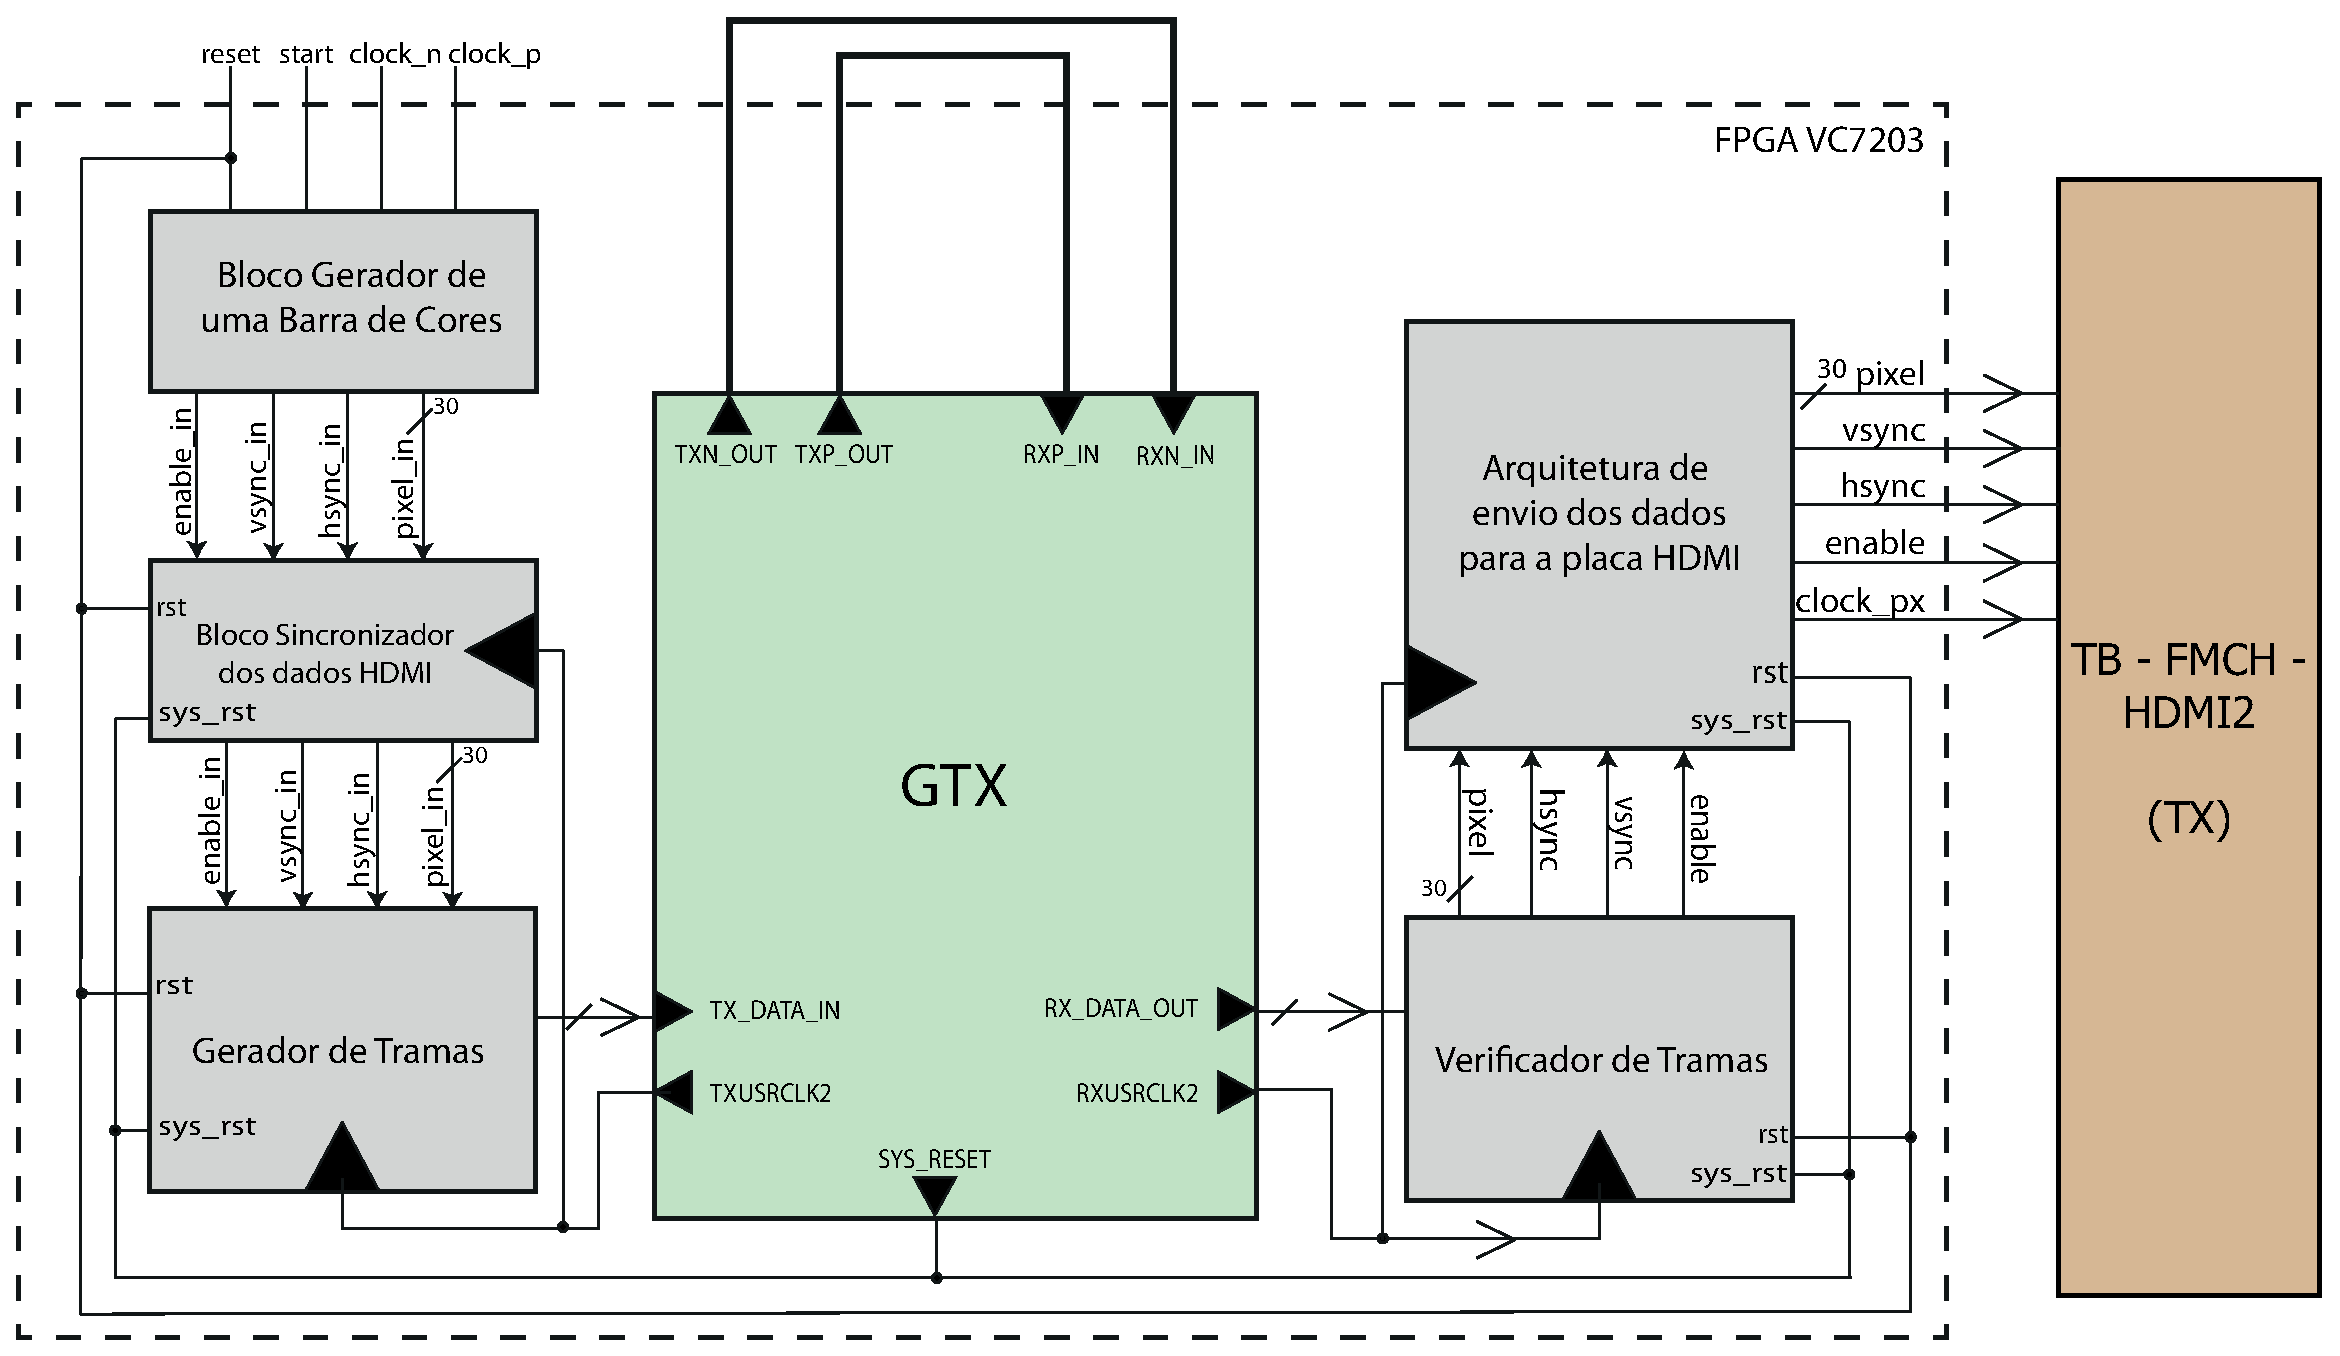
\includegraphics[width=1.0\textwidth]{planod_simples}
		\captionsetup{width=1.0\linewidth}
		\caption[Diagrama de blocos geral da arquitetura que transmite uma barra de cores em série]{Diagrama de blocos geral da arquitetura que transmite uma barra de cores em série}
		\label{fig:planD_SIMPLES}
	\end{center}
\end{figure}

Tal como é de esperar e foi referido em \ref{sec:sincronizacao} na página \pageref{sec:sincronizacao}, os sinais de relógio provenientes do GTX e do módulo que gera a barra de cores não são o mesmo, e por isso, existe um bloco entre a geração e a criação de tramas que permite a sincronização entre os diferentes domínios de sinais de relógio através de \textit{shift-registers}.

Tendo em conta a arquitetura global desenvolvida foram tomadas duas decisões importantes para definir as características do transcetor: o número de bits por trama e a frequência a que estas serão lidas para o mesmo. Tal como referido anteriormente, a maneira mais eficiente no que toca à escolha da frequência de amostragem para o transcetor, é escolher a própria frequência da imagem HDMI, ou seja, \SI{148.5}{\mega\hertz} para uma imagem \textit{FULL HD}. Relativamente ao número de bits por trama, tendo em conta que é necessário enviar os sinais todos (\textit{pixel}, \textit{vsync}, \textit{hsync} e \textit{enable}) e visto que nesta fase do projeto não houve a preocupação da criação de diferentes tramas para os diversos momentos de transmissão, escolheu-se enviar tramas de 40 bits.

Observando novamente a tabela \ref{table:line_rates} conclui-se que, independentemente do tamanho do \textit{datapath} escolhido, obtém-se uma taxa de transmissão de dados de \SI{5.94}{\giga\bit\per\second}.

\subsubsection{Geração do Módulo GTX} \label{subsub:GTX_generate}

Quando se gera o módulo GTX através da interface disponibilizada pelo \textit{software} VIVADO existem algumas decisões que necessitam de ser tomadas para além das que já foram mencionados. Essas passam de seguida a ser detalhadas:

Do lado do transmissor tomaram-se as seguintes principais decisões:
\begin{enumerate}
%	\item \textbf{\textit{Line Rate:}} Como referido anteriormente é 5,94 Gb/s.
%	\item \textbf{Frequência de Amostragem das Tramas:} Assim como referido anteriormente é 148,5 MHz.
%	\item \textbf{Tamanho da interface com a FPGA:} Tal como explicado em \ref{subsub:planD_considerações} na página \pageref{subsub:planD_considerações} é 40 bits
	\item \textbf{Tamanho interno dos dados:} Esta escolha envolve o número de caminhos de dados (\textit{datapath}) que são utilizados e ainda o valor da frequência de TXUSRCLK. Escolheu-se 40 bits para tal, o que implica o uso de apenas um \textit{datapath}, obtendo-se as frequências idênticas de TXUSRCLK e TXUSRCLK2.
	\item \textbf{Tipo de codificação:} Neste caso não se escolheu codificação porque não é possível (a interface com a FPGA é de 40 bits) e também numa fase inicial optou-se por simplificar o projeto.
	\item \textbf{Escolha ente \textit{Buffer} ou Bloco de Alinhamento de Fase:} Tal como indicado na secção \ref{subsub:tx_buffer}, foi escolhido a utilização do \textit{buffer} uma vez que é de mais fácil utilização não requerendo o uso de lógica extra (comparativamente ao bloco de alinhamento de fase) e ainda assim é robusto.
\end{enumerate}

Do lado do recetor as principais decisões tomadas foram as seguintes:
\begin{enumerate}
	\item \textbf{Tipo de equalização:} Na subsecção \ref{subsub:rx_equalização} são apresentadas as vantagens de cada um dos tipos de equalizadores disponíveis. Apesar de este ser um projeto simples em que não se pretende inserir o sinal em canais ruidosos, optou-se por utilizar um equalizador DFE uma vez que traz mais vantagens do que a utilização do equalizador LPM.
	
	\item \textbf{Alinhamento de palavras:} Como palavra de alinhamento escolheu-se o símbolo K28.3 da tabela \ref{table:caracteres_especiais_8b10b}. Contudo, é necessário ter em conta que não se está a utilizar codificação e, como tal, para efetuar o alinhamento da palavra o recetor não alinha pelo símbolo K28.3 codificado, mas sim, não codificado. Ou seja, na realidade quando encontrar a palavra "7C" assume que é a palavra de alinhamento e a trama passa a estar alinhada para esse limite. Para além disso, optou-se por ativar a porta "RXSLIDE" que ativa o alinhamento manual dos bits, pois tal como referido em \ref{subsub:align} é de esperar que seja necessário ativar o alinhamento manual para ligações cuja taxa de débito seja superior a \SI{5}{\giga\bit\per\second}.
	
	\item \textbf{Tipo de descodificação:} Não foi utilizada nenhuma descodificação, pois do lado do transmissor também não há codificação.
	\item \textbf{Escolha ente \textit{Buffer} ou Bloco de Alinhamento de Fase:} Optou-se pela escolha do \textit{buffer}, porque no caso do recetor para além não requerer lógica extra e ter uma inicialização mais rápida (comparativamente ao bloco de alinhamento de fase), também não exige que a correção do sinal de relógio seja realizada fora do transcetor, tal como mencionado em \ref{subsub:rx_buffer}.
\end{enumerate}

\begin{table}[h!]
	\centering
	\caption[Sumário do módulo GTX gerado para a transmissão em série de uma barra de cores gerada na FPGA]{Sumário do módulo GTX gerado para a transmissão em série de uma barra de cores gerada na FPGA (adaptada do \textit{software})}
	\label{table:sumario_planoD}
	\begin{tabular}{@{}ll@{}}
		\toprule
		\multicolumn{1}{c}{\textbf{Característica}} & \multicolumn{1}{c}{\textbf{GT}} \\ \midrule
		\textbf{TX Line Rate (Gbit/s)}                & \num{5,94}                            \\
		\textbf{TX Reference Clock (MHz)}           & \num{148.5}                         \\
		\textbf{Enconding}                          & None                            \\
		\textbf{TX Internal Data Width}             & 40                              \\
		\textbf{TX External Data Width}             & 40                              \\
		\textbf{TXUSRCLK (MHz)}                     & 148,5                           \\
		\textbf{TXUSRCLK2 (MHz)}                    & 148,5                           \\
		\textbf{TX Buffer Enabled}                  & TRUE                            \\
		\textbf{RX Line Rate (Gbit/s)}                & \num{5,94}                            \\
		\textbf{RX Reference Clock (MHz)}           & \num{148.5}                           \\
		\textbf{Decoding}                           & None                            \\
		\textbf{RX Internal Data Width}             & 40                              \\
		\textbf{RX External Data Width}             & 40                              \\
		\textbf{RXUSRCLK (MHz)}                     & \num{148.5}                           \\
		\textbf{RXUSRCLK2 (MHz)}                    & \num{148.5}                           \\
		\textbf{RX Buffer Enabled}                  & TRUE                            \\ \bottomrule
	\end{tabular}
\end{table}

Na tabela \ref {table:sumario_planoD} é apresentada uma tabela sumário do módulo gerado. Esta tabela foi adaptada da interface que gera o módulo.

\subsubsection{Conceção e Desenvolvimento}

Na figura \ref{fig:planD_SIMPLES} é representado um diagrama de blocos geral da arquitetura apresentada. Nesta subsecção são detalhados todos os blocos utilizados e suas entradas e saídas para que se possa perceber as ligações entre os mesmos. 

\subsubsection*{Bloco gerador de uma Barra de Cores} \label{subsub:serial_colorBarGenerator}

Este bloco gerador de barra de cores é exatamente igual ao bloco descrito em \ref{subsub:planA}: gera uma barra de cores em \textit{FULL HD} com uma frequência de \SI{148.5}{\mega\hertz}. Nas suas entradas encontram-se as portas vindas diretamente do exterior, tal como nas outras arquiteturas que utilizam este bloco. Estas são os botões definidos pelo utilizador (\textit{reset} e \textit{start}) e também um sinal de relógio diferencial de \SI{200}{\mega\hertz}. Nas suas saídas encontram-se os sinais referentes à imagem gerada que são posteriormente enviados para um bloco sincronizador dos dados HDMI.

\subsubsection*{Bloco Sincronizador dos dados HDMI} \label{subsub:serial_syncsignals}

O recurso a este bloco sincronizador dos dados HDMI deve-se aos diferentes domínios de relógio que existem no sistema: por um lado existe um bloco que gera uma barra de cores a uma determinada cadência, e por outro existe um bloco que gera as tramas a serem enviadas para o transcetor a outra cadência. Estes dois sinais de relógio podem ser iguais, no entanto podem não estar em fase o que é suficiente para haver problemas de meta-estabilidade. 

Por este motivo, este bloco de sincronização é apenas constituído por dois registos de deslocamento (\textit{shift-registers}) para que problemas de sincronização que possam eventualmente existir sejam resolvidos. O diagrama de blocos deste módulo é apresentado na figura \ref{fig:sync_block}. 

\begin{figure}[h!]
	\begin{center}
		\leavevmode
		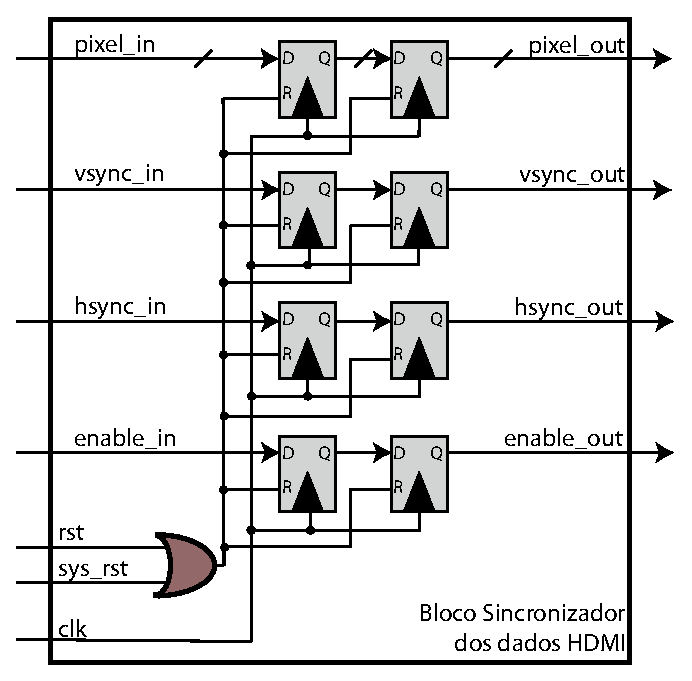
\includegraphics[width=0.5\textwidth]{sync_block_from_HDMI}
		\captionsetup{width=1.0\linewidth}
		\caption[Bloco de sincronização de dados]{Bloco de sincronização de dados}
		\label{fig:sync_block}
	\end{center}
\end{figure}

Tal como se visualiza na figura, para além de nas suas entradas se encontrar os dados provenientes da fonte HDMI há também dois sinais : \textit{rst} e \textit{sys\_rst}. O primeiro sinal refere-se ao sinal de \textit{reset} controlado pelo utilizador e o segundo corresponde a um sinal de \textit{reset} ativado automaticamente pelo módulo GTX.

O sinal de relógio a que opera este bloco trata-se do sinal de relógio proveniente do módulo GTX, tal como se visualiza na figura \ref{fig:planD_SIMPLES}.

\subsubsection*{Gerador de Tramas} \label{subsub:serial_frameGenerator}

Este bloco é responsável pela criação das tramas a serem enviadas para o módulo GTX. Relembra-se que nesta abordagem inicial do projeto não se teve em conta a criação de tramas bem definidas para todos os momentos de transmissão. 

Definiu-se a trama correspondente ao início da transmissão para que seja possível manter o alinhamento do lado do recetor e iniciar o processo. Esta é designada por  SOP (\textit{Start of Packet}) e é enviada em momentos de transmissão nulos, ou seja, quando os sinais de controlo da imagem se encontram inativos ($vsync = 0$, $hsync = 0$ e $enable = 0$), sendo constituída por 40 bits que em hexadecimal corresponde a: 000605047c. Este padrão sugerido pelo exemplo disponibilizado no \textit{software} da \textit{Xilinx} possui as seguintes particularidades:

\begin{enumerate}
	\item No final da mesma encontra-se a palavra de alinhamento (conjunto dos primeiros bits a ser transmitido) que permite ao transcetor alinhar a trama internamente.
	\item Nunca será confundida como trama de informação (apresentada na figura \ref{fig:trama_abordagem_inicial}) devido à composição dos últimos 7  bits de ambas. A trama SOP termina em 1111100, e a trama de informação termina em 1010101.
\end{enumerate}



%%Explicar como são os pacotes noutras alturas de transmissão sem ser qdo se envia SOP
Quando algum sinal de controlo referente à imagem está ativo é transmitida uma trama de informação com o formato que se visualiza na figura \ref{fig:trama_abordagem_inicial}.

\begin{figure}[h!]
	\begin{center}
		\leavevmode
		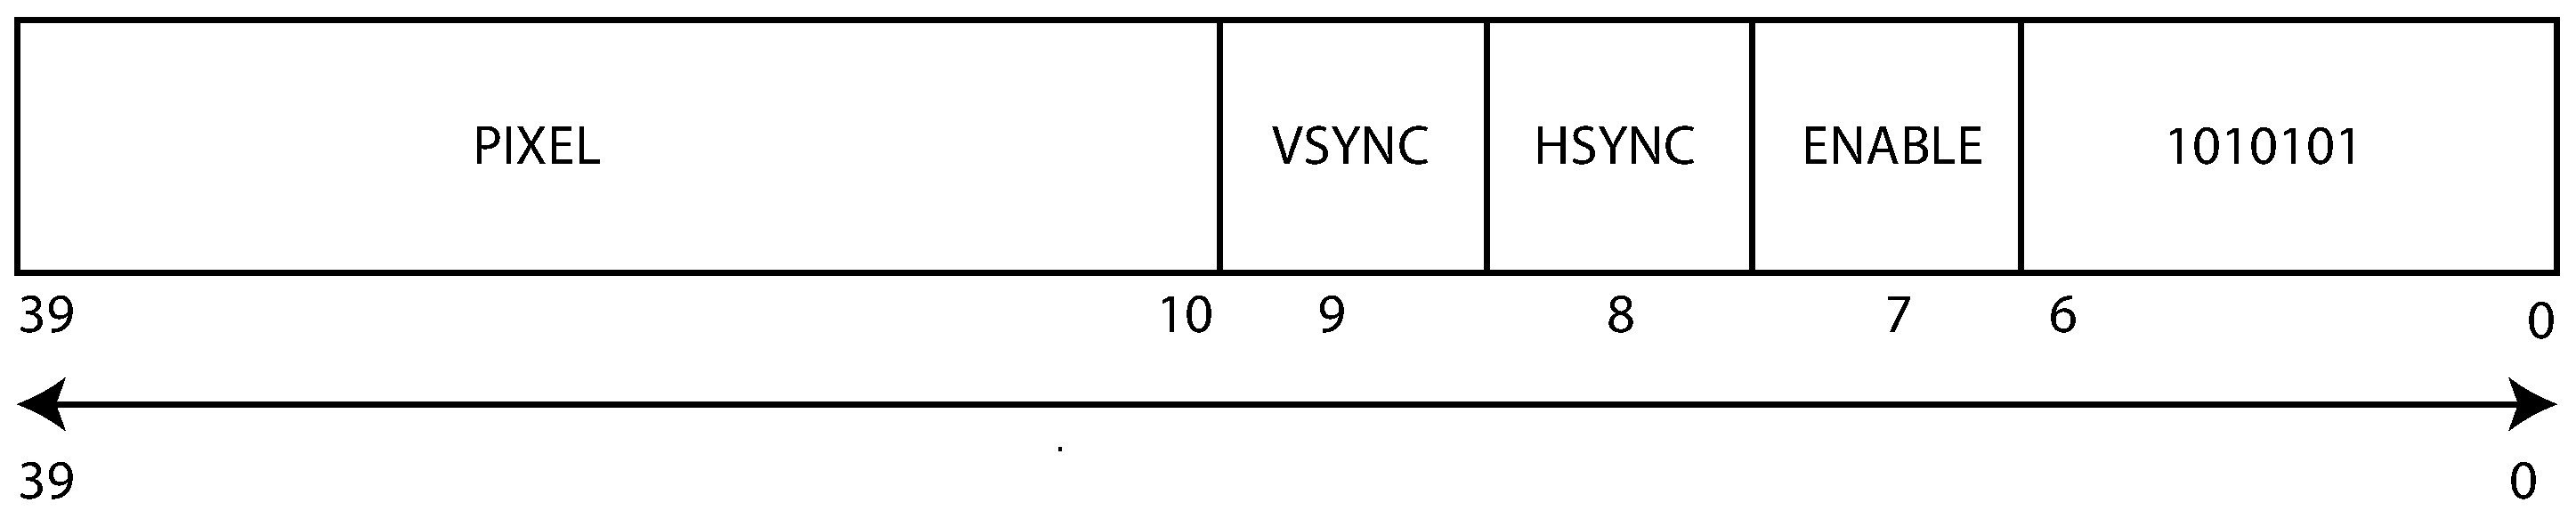
\includegraphics[width=0.9\textwidth]{trama_abordagem_inicial}
		\captionsetup{width=1.0\linewidth}
		\caption[Estrutura das tramas de informação]{Estrutura das tramas de informação}
		\label{fig:trama_abordagem_inicial}
	\end{center}
\end{figure}

Assim sendo, consoante os dados que recebe nas suas entradas (\textit{pixel}, \textit{vsync}, \textit{hsync} e \textit{enable}), este bloco ou envia SOP ou envia tramas de informação. A figura \ref{fig:momentos_tramas} exemplifica os diversos momentos de transmissão das diferentes tramas numa imagem. A cinza correspondem os momentos da imagem em que os sinais de controlo da mesma estão inativos, e por isso são transmitidas tramas SOP. A castanho correspondem os momentos de transmissão em que algum dos sinais de controlo de imagem está ativo e por isso são enviadas tramas de informação. Sempre que o sinal \textit{rst} ou \textit{sys\_rst} estiver ativo os dados são repostos e as tramas enviadas são SOP. 

\begin{figure}[h!]
	\begin{center}
		\leavevmode
		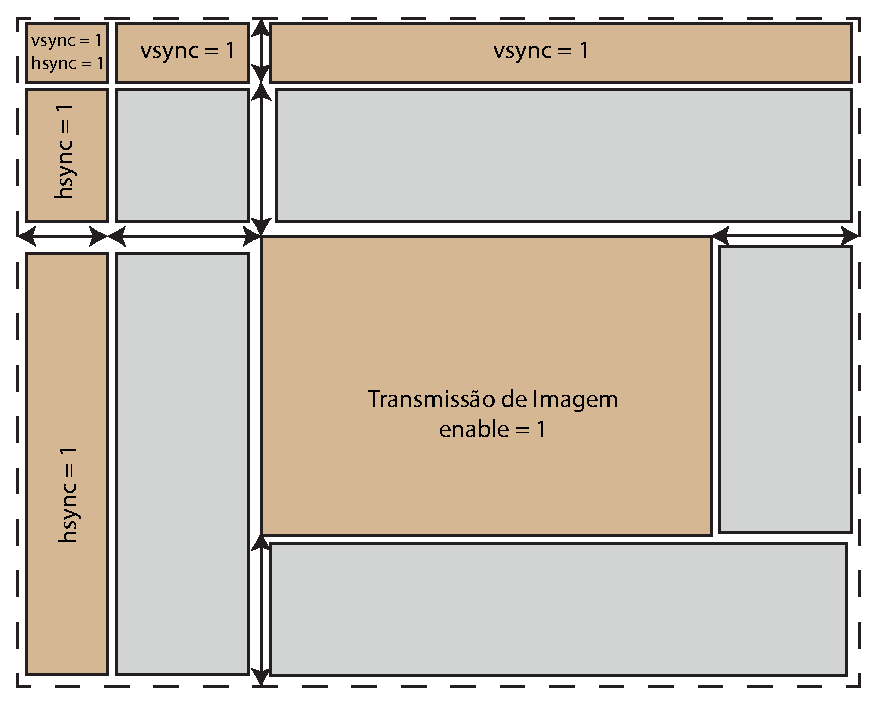
\includegraphics[width=0.7\textwidth]{exemplo_tramas_transmissoes}
		\captionsetup{width=1.0\linewidth}
		\caption[Momentos de transmissão de diferentes tramas]{Momentos de transmissão de diferentes tramas}
		\label{fig:momentos_tramas}
	\end{center}
\end{figure}

É de esperar que a transmissão demore algum tempo a alinhar do lado do recetor, sendo necessário que as tramas SOP sejam enviadas durante algum tempo. Por este motivo escolheram-se os momentos de transição de dados de controlo nulos, pois são suficientemente longos para que a transmissão possa ser alinhada. Assim, no pior dos casos, perde-se a primeira imagem completa que é transmitida, pois não são recebidos os primeiros dados de controlo (\textit{vsync} e \textit{hsync}) mas garante-se que todas as outras estão alinhadas e os dados serão corretamente recebidos do lado do transmissor.

\subsubsection*{Verificador de Tramas} \label{subsub:serial_frameChecker}
  
%%Explicar porque existe

Este bloco é responsável pela re-organização das tramas recebidas que são recebidas à cadência RXUSRCLK2. Apesar de poder parecer que com o alinhamento interno as tramas chegariam ao recetor tal como são enviadas do transmissor, isso raramente se verifica. As tramas são alinhadas para um determinado limite assim que o recetor encontra a palavra de alinhamento. %, no entanto não significa que a trama recebida é exatamente igual à trama enviada. 

Segundo \cite{R022} e \cite{R011}, quando a palavra de alinhamento é detetada no recetor, este assume que os dados a partir daí são válidos e alinha-os para um determinado limite. Este limite pode ser selecionado aquando a criação do módulo GTX, tendo-se optado por alinhar os dados para o \textit{byte} mais próximo. Apesar de não se estar a lidar com codificação e devido ao tamanho do \textit{datapath} ser 40 bits, o bloco de alinhamento das palavras considera que 1 \textit{byte} são 10 bits (a codificação 8B/10B codifica 8 bits em 10 bits). Assim, quando é detetada a palavra de alinhamento as tramas recebidas no recetor podem chegar de quatro maneiras diferentes ilustradas na figura \ref{fig:alinhamento_tramas_gtx}.


%Se o datapath fosse de 32 bits sem codificação, assumiria que 1 \textit{byte} sao 8 bits, de certeza, apesar de eu nao ter testado
\begin{figure}[h!]
		\begin{center}
		\leavevmode
		\includegraphics[width=0.8\textwidth]{organizacao_tramas}
		\captionsetup{width=1.0\linewidth}
		\caption[Alinhamento das tramas no transcetor]{Alinhamento das tramas no transcetor}
		\label{fig:alinhamento_tramas_gtx}
	\end{center}
\end{figure}

Daí a importância da trama de SOP: quando é detetada em algum dos limites assinalados a cinzento dá-se início à transmissão dos restantes dados. Para se proceder à organização dos dados recebidos é necessário recorrer a uma máquina de estados. Esta foi adaptada da que a ferramenta de \textit{software} cria por omissão quando é gerado um exemplo deste módulo GTX.

A máquina de estados principal é dividida em três por questões de simplificação e de melhor entendimento da mesma. Cada uma destas divisões passa a ser detalhada, sem nunca esquecer que funcionam como um todo.
%%Explicar máquina de estados que procura dados, ou espera ou tal e tal

\begin{enumerate}
	\item \textbf{Máquina de estados geral da receção de dados:}
	
	Esta máquina é composta por três estados que definem o estado geral da receção de dados. Estes estados são:
	\begin{itemize}
		\item \textbf{\textit{Begin:}} Estado inicial que aguarda a receção de dados válidos do recetor. Quando a trama de SOP é detetada pela primeira vez, então a máquina transita para um estado em que recebe dados válidos. 
		
		\item \textbf{\textit{Track\_data:}} Neste estado já foi detetato o início da transmissão (SOP) e por isso todos os dados que estão a ser recebidos são considerados válidos. Quando é detetado algum erro (com a ajuda de uma máquina de estados detetora de erros) transita de estado.
		
		\item \textbf{\textit{Data\_error\_detected:} }Estado de deteção de erro que transita imediatamente para o estado inicial para aguardar a chegada de dados válidos novamente.
		
	\end{itemize}

	Sempre que for necessário fazer \textit{reset} ao sistema, quer pela ativação do utilizador ou então pelo transcetor, volta-se ao estado inicial "\textit{begin}".
	
	
	\begin{figure}[h!]
		\begin{center}
			\leavevmode
			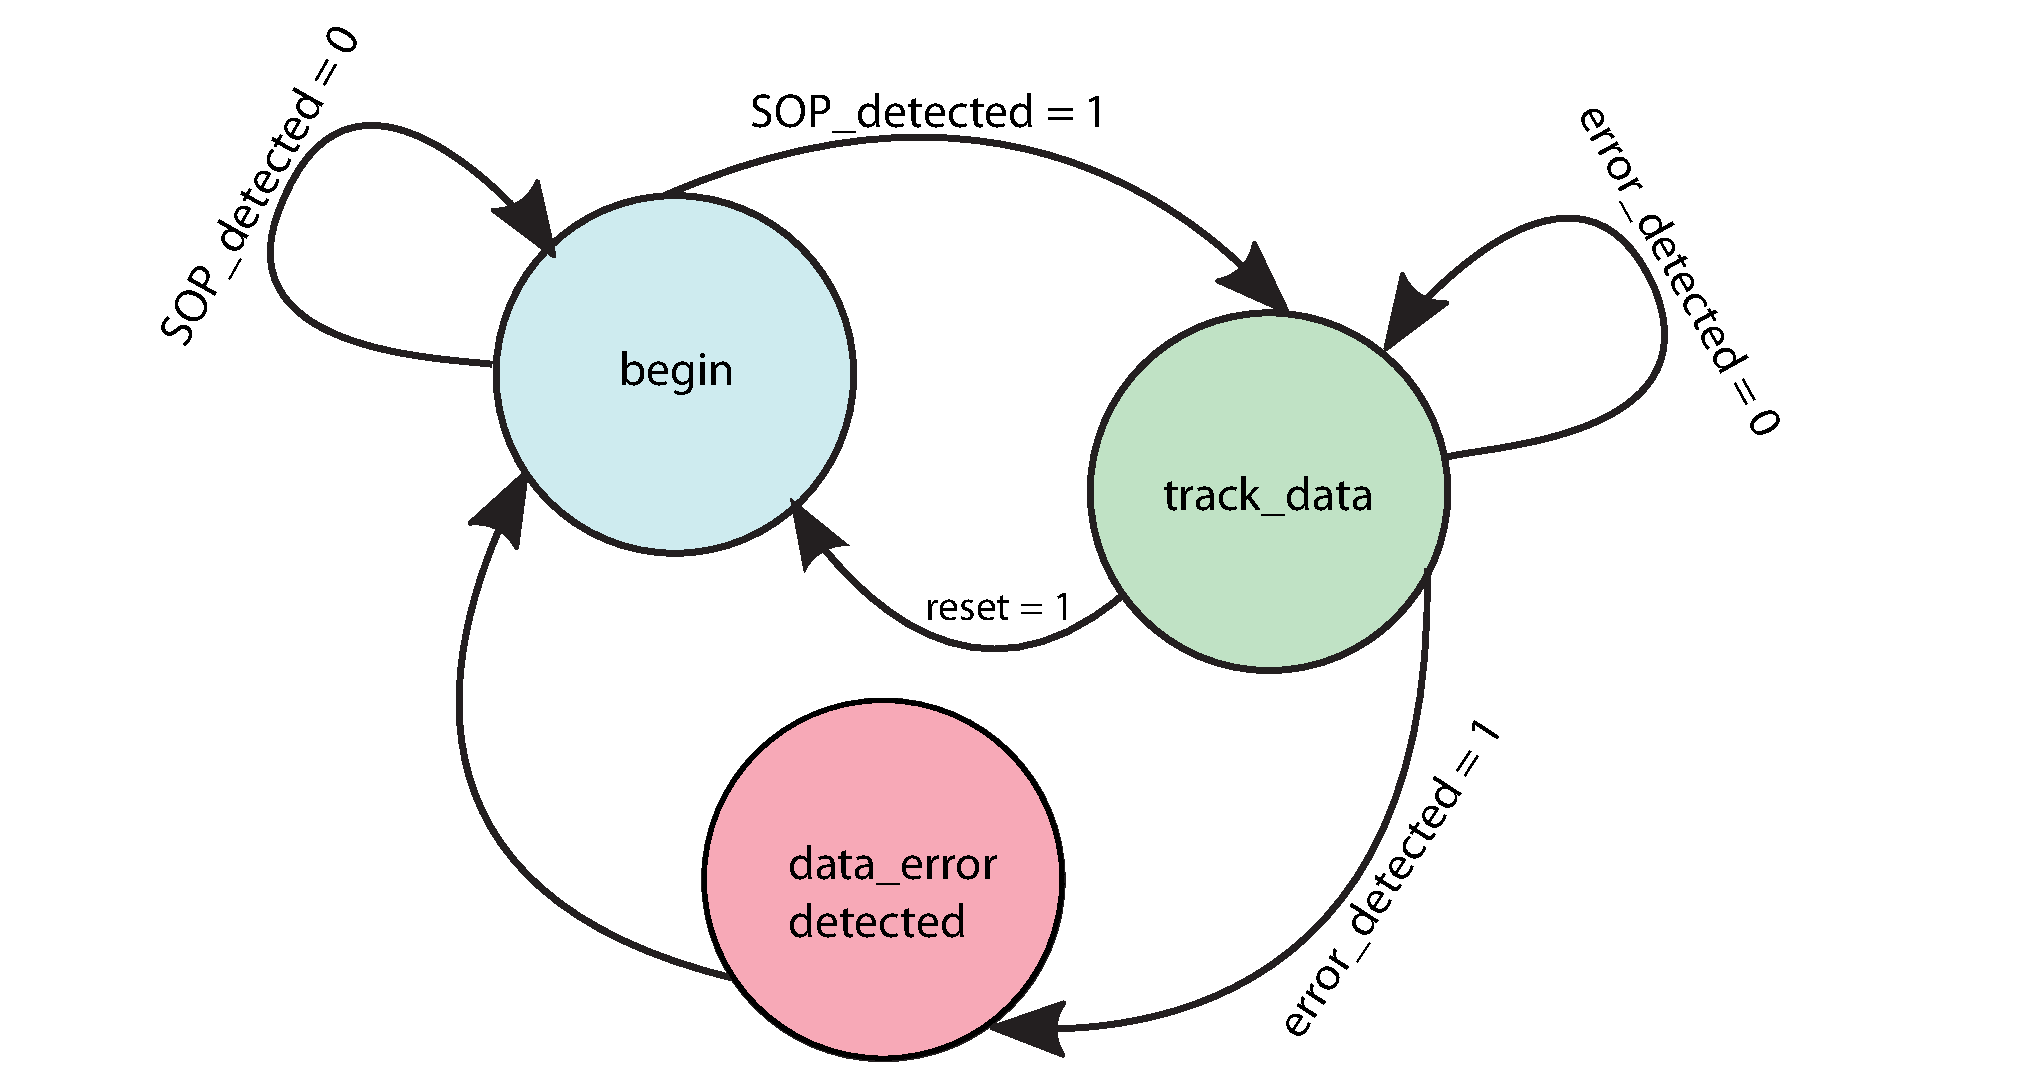
\includegraphics[width=0.8\textwidth]{fsm1}
			\captionsetup{width=1.0\linewidth}
			\caption[Máquina de estados de transmissão]{Máquina de estados de transmissão}
			\label{fig:FSM1}
	\end{center}
	\end{figure}
	
	A figura \ref{fig:FSM1} representa a máquina de estados detalhada anteriormente. De notar que na imagem estão representadas algumas \textit{flags} de decisão de transição de estados. A \textit{flag} "\textit{SOP\_detected}" indica que se a trama de início de pacote foi encontrada nos dados recebidos e "\textit{error\_detected}" indica que foi detetado um erro nos dados recebidos. Ambas são definidas por máquinas de estados que serão explicadas mais adiante.
	
	
	\item \textbf{Máquina de leitura de dados}
	 
	 Esta máquina de estados é responsável pela constante procura de dados recebidos pelo recetor. Destes apenas são guardadas as últimas duas tramas porque da sua combinação resulta a indicação de início de transmissão, iniciando o funcionamento desta máquina de estados.
	 
	 A figura \ref{fig:fsm2} ilustra a máquina de estados aqui referida, contudo antes de se detalhar os diferentes estados da mesma, faz-se uma breve descrição das \textit{flags} de transição de estados presentes na figura:

	 	\begin{figure}[h!]
	 		\begin{center}
	 			\leavevmode
	 			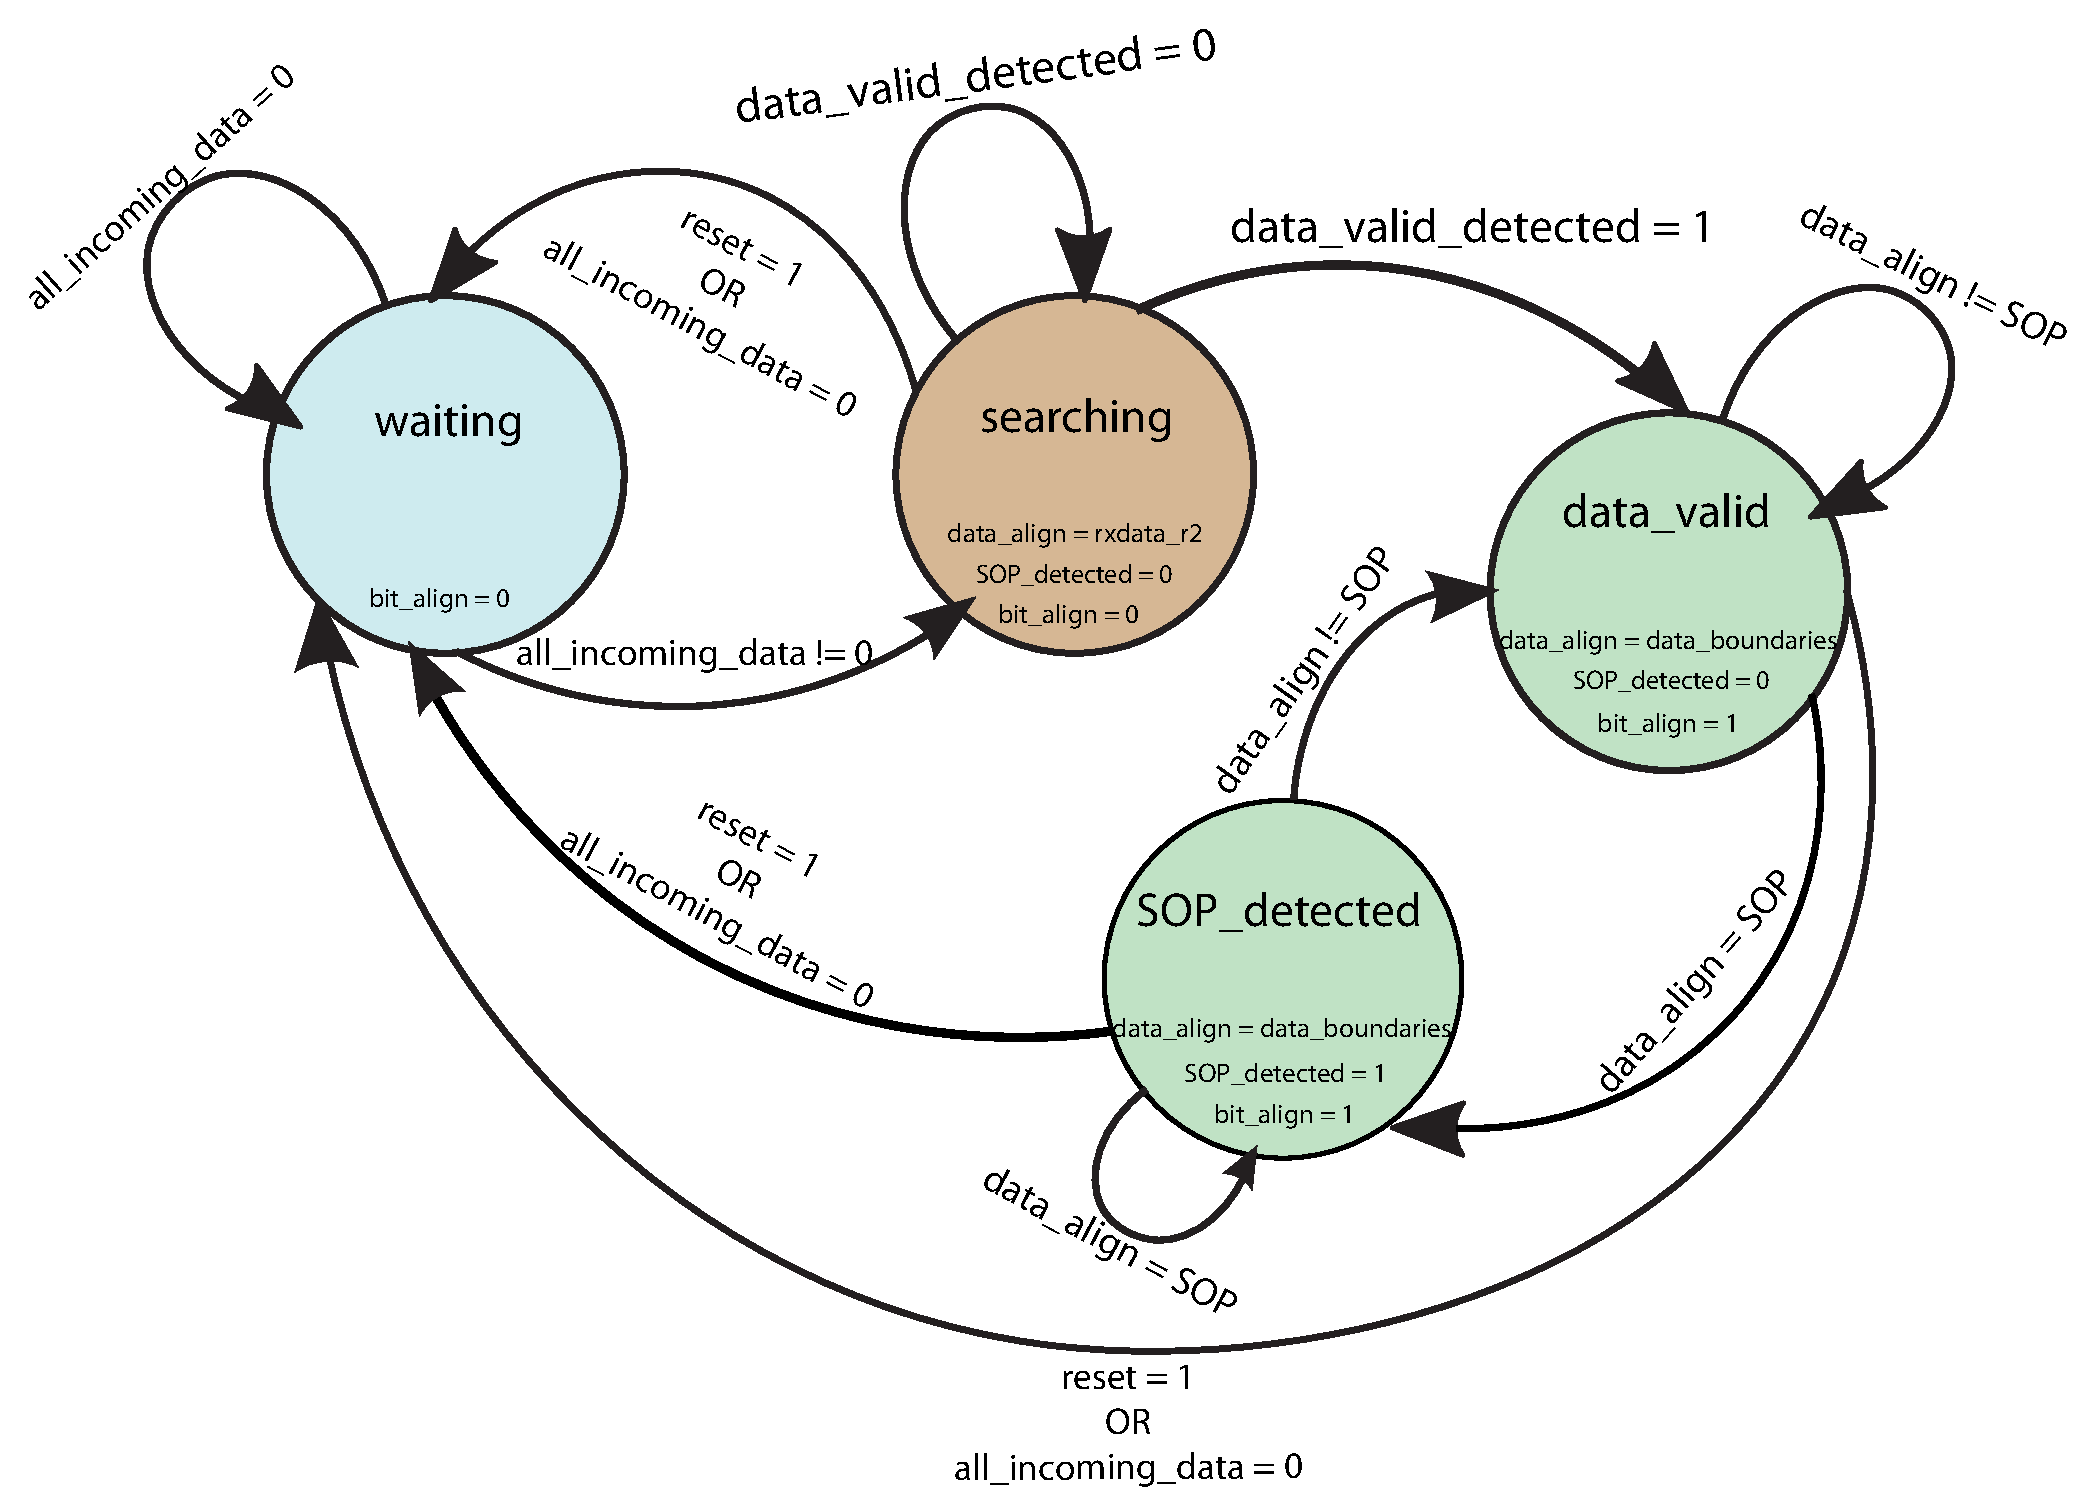
\includegraphics[width=0.8\textwidth]{fsm_track_data}
	 			\captionsetup{width=1.0\linewidth}
	 			\caption[Máquina de estados leitura de dados]{Máquina de estados leitura de dados}
	 			\label{fig:fsm2}
	 		\end{center}
		\end{figure}
	 
	\begin{itemize}
		\item \textit{all\_incoming\_data}: Esta \textit{flag} indica se todos os bits presentes nas duas últimas tramas recebidas no recetor são 0 ou não. Se sim, então a \textit{flag} é igual zero, senão é um.
		
		\item \textit{data\_valid\_detected}: Esta \textit{flag} indica se foi encontrado nos dados recebidos (nas duas últimas tramas) a trama SOP em alguma das situações assinaladas a cinza presentes na figura \ref{fig:alinhamento_tramas_gtx}.
		
		\item \textit{reset}: indica se foi ativado o sinal para repôr os dados originais da máquina de estados.
	\end{itemize}	 
	 
	 Estas são as principais \textit{flags} de transição de estados da máquina. De seguida serão detalhados todos os estados da mesma:
	 
	 	 \begin{itemize}
	 	\item \textbf{\textit{Waiting}:} Este estado indica que o recetor ainda não está a receber dados, isto porque a \textit{flag} \textit{all\_incoming\_data} está inativa. Por defeito, quando não há transmissão de dados do lado do transmissor, o recetor recebe apenas dados iguais a zero. Assim que esta \textit{flag} se ativa então passa-se para o estado \textit{searching}.
	 	
	 	\item \textbf{\textit{Searching}:} Neste estado, a máquina procura a trama que dá inicio à transmissão de dados (SOP). Uma vez que ela pode vir alinhada em diferentes \textit{bytes} nas tramas do recetor, então a máquina procura a SOP nas quatro situações apresentadas na figura \ref{fig:alinhamento_tramas_gtx}. Assim que encontra SOP, memoriza os limites das tramas em que esta foi encontrada para que se possa retirar todos os outros dados de transmissão e transita de estado.
	 	
	 	\item \textbf{\textit{Data\_valid}:} Este estado serve essencialmente para guardar os dados devidamente alinhados segundo os limites da trama SOP. Ativa-se a flag \textit{bit\_align} para que o sistema reconheça que os dados se encontram alinhados. Se os dados que estão a ser guardados em \textit{data\_align} corresponderem à trama SOP então transita-se de estado para indicar que esta trama foi detetada. 
	 	
	 	\item \textbf{\textit{SOP\_detected}:} Quando este estado está ativo, então os dados alinhados correspondem à trama SOP, e por isso deve-se ativar a \textit{flag} "\textit{SOP\_detected}". Este estado mantém-se ativo enquanto os dados alinhados corresponderem à trama SOP e transita para o estado "\textit{data\_valid}" assim que tal deixar de ser verdade. 
	 \end{itemize}
 
 		Sempre que a transmissão for interrompida (\textit{all\_incoming\_data} se iguala a zero) ou o sinal de \textit{reset} for ativo (quer por opção do utilizador ou pelo módulo GTX), então a máquina retorna ao estado inicial e repõe os dados originais do sistema. 
	 
	 	Inicialmente o estado ativo é "\textit{waiting}", e todas as \textit{flags} de decisão de mudança de estado (\textit{all\_incoming\_data} e \textit{data\_valid\_detected}) estão igualadas a zero.
	 
	 
	 \item \textbf{Máquina de estados de verificação do alinhamento dos dados}
	
	Tal como já foi mencionado anteriormente, para taxas de transmissão superiores a \SI{5}{\giga\bit\per\second} , o transcetor pode alinhar falsamente os dados. Por esse motivo, as tramas recebidas podem não vir dentro dos limites apresentados na figura \ref{fig:alinhamento_tramas_gtx}, sendo assim necessário o recurso a uma máquina de estados que valide o correto alinhamento.
	
	A máquina de estados apresentada na figura \ref{fig:fsm3} é responsável pela deteção do devido alinhamento das tramas recebidas de acordo com a figura \ref{fig:alinhamento_tramas_gtx}. Caso tal não se verifique procede ao alinhamento manual das tramas.
	
		\begin{figure}[h!]
			\begin{center}
				\leavevmode
				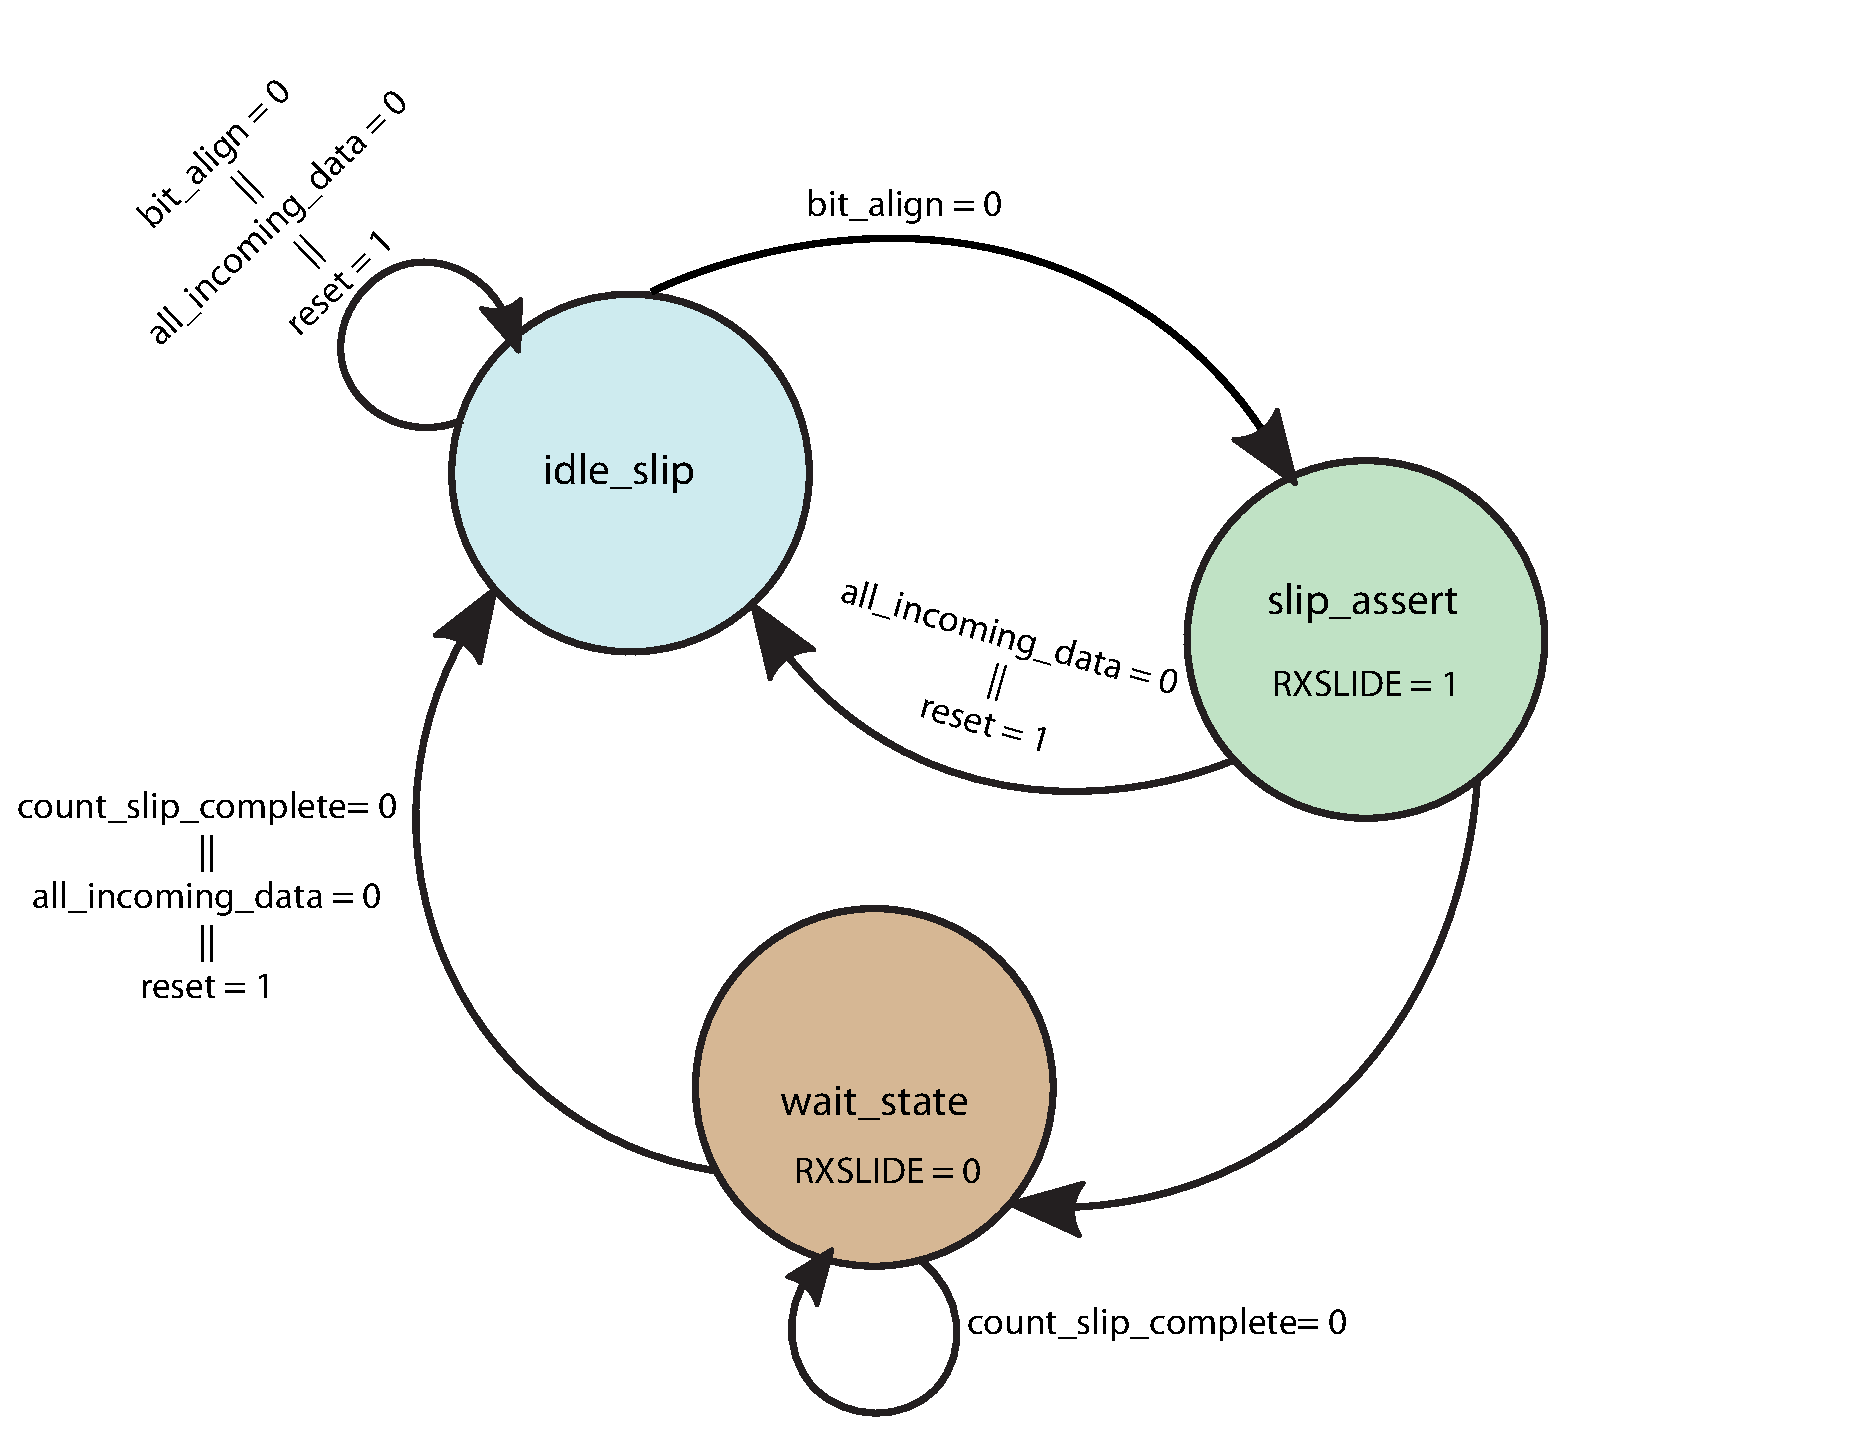
\includegraphics[width=0.9\textwidth]{fsm_bit_align}
				\captionsetup{width=1.0\linewidth}
				\caption[Máquina de estados de verificação do alinhamento dos dados]{Máquina de estados de verificação do alinhamento dos dados}
				\label{fig:fsm3}
		\end{center}
	\end{figure}
	
	%Descrição das flags
	Antes de se passar à descrição de cada estado, é de notar que existem algumas \textit{flags} de decisão de transição de estados:
	\begin{itemize}
		\item \textit{bit\_align}: Esta \textit{flag} indica se a palavra se encontra devidamente alinhada, tal como ilustrada na figura \ref{fig:alinhamento_tramas_gtx}. 
		
		\item \textit{all\_incoming\_data}: Esta \textit{flag} já foi mencionada e detalhada na máquina de estado que faz a leitura de dados.
		
		\item \textit{count\_slip\_complete}: Esta é uma \textit{flag} que fica ativa quando um contador termina (será explicado mais à frente).
		
		\item \textit{reset}: Indica a reposição dos dados originais da máquina de estados quando ativa.
	\end{itemize}
	
	%Descrição dos estados
	
	Esta máquina é composta por três estados, sendo estes:
	\begin{itemize}
		\item \textbf{\textit{Idle\_slip}:} Este estado aguarda pela receção de dados e também pela deteção do desalinhamento da palavra. Há transição de estado quando se verifica que as tramas que chegam ao recetor não estão alinhadas de acordo com os limites que deveriam estar.
		
		\item \textbf{\textit{Slip\_assert}:} Este estado está ativo quando há deteção de falso alinhamento de palavras, e por isso a saída que se conecta ao GTX é ativada: RXSLIDE. A ativação deste sinal vai permitir que as tramas sejam deslocadas em 1 bit. Este estado transita imediatamente para o estado de \textit{Wait\_state}.
		
		\item \textbf{\textit{Wait\_state}:} Neste estado o sinal de saída RXSLIDE volta a estar inativo e aguarda-se que a operação de deslocamento de 1 bit se verifique. Como estamos perante um \textit{datapath} de 40 bits, segundo \cite{R011} aguarda-se 64 ciclos de relógio. Após esta espera, a flag \textit{count\_slip\_complete} fica ativa e há transição de estado.
	\end{itemize}
	
	De notar que sempre que houver falha de transmissão ou o sinal de \textit{reset} for ativo, os sinais são repostos para os originais e volta-se ao estado \textit{Idle\_slip}.
	
	%Descrição dos dados originais da maquina
	
	Inicialmente o estado ativo é o {\textit{Idle\_slip} }e as \textit{flags} de sinalização de transição de estado são igualadas a 0.
	
%	\item \textbf{Máquina que deteta os erros }
%	\item \textbf{Máquina que deteta o estado da ligação}
\end{enumerate}

Para além destas máquinas de estados apresentadas existe a possibilidade de implementação de uma outra que verifique os erros das tramas recebidas. Esta máquina torna-se útil quando há implementação de códigos detetores de erros nas tramas, ativando a \textit{flag}  "\textit{error\_detected}", sempre que o \textit{checksum} recebido na trama não corresponder à mensagem. Contudo, nesta abordagem inicial tal não é realizado e por isso essa \textit{flag} é globalmente igualada a zero.

Quando os dados estão alinhados procede-se à extração da informação contida na trama recebida, enviando-a para o bloco responsável pela sua transmissão para a placa HDMI, sendo necessário que o estado  \textit{track\_data} esteja ativo. A informação retirada depende do tipo de trama recebida: caso a trama seja SOP, os dados são todos igualados a 0; caso contrário, então extrai-se os dados de acordo com o formato da trama de informação apresentado na figura \ref{fig:trama_abordagem_inicial}.


%Se a trama recebida é uma SOP, igualam-se todos os dados a zero. Caso 
%
%Quando se recebe uma trama que é igual a SOP iguala-se todos os sinais a zero, no entanto quando a ligação está a procura de dados (o estado \textit{track\_data} está ativo) os dados são extraídos segundo o formato da trama enviada , representada na imagem  na página \pageref{fig:trama_abordagem_inicial}.

\subsubsection*{Bloco de envio de dados para a placa HDMI} \label{subsub:serial_send signals to HDMI}

Este bloco é responsável pela receção dos dados alinhados provenientes do bloco verificador de tramas e do seu posterior envio para a placa HDMI transmissora. A figura \ref{fig:sync_block_to_HDMI} é apresentado o diagrama de blocos deste módulo.

\begin{figure}[h!]
	\begin{center}
		\leavevmode
		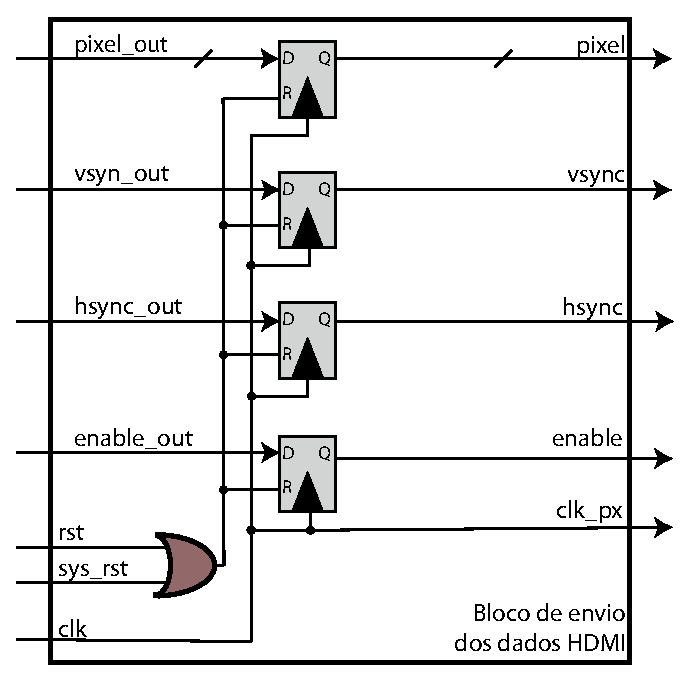
\includegraphics[width=0.5\textwidth]{sync_block_to_HDMI}
		\captionsetup{width=1.0\linewidth}
		\caption[Diagrama de blocos de envio de dados para a placa HDMI transmissora]{Diagrama de blocos de envio de dados para a placa HDMI transmissora}
		\label{fig:sync_block_to_HDMI}
	\end{center}
\end{figure}

Os dados recebidos neste bloco são lidos para um registo ao flanco positivo do sinal de relógio que alimenta este módulo (RXUSRCLK2). Posteriormente, todos os dados presentes nos registos são enviados para a placa HDMI transmissora incluindo o sinal de relógio RXUSRCLK2.

\subsubsection*{Localizações das portas de saída do módulo de topo} \label{subsub:serial_locs_planD}

Na figura \ref{fig:planD} visualiza-se o diagrama de blocos desenvolvido para esta arquitetura com os seus diversos sub-módulos. 
\begin{figure}[h!]
	\begin{center}
		\leavevmode
		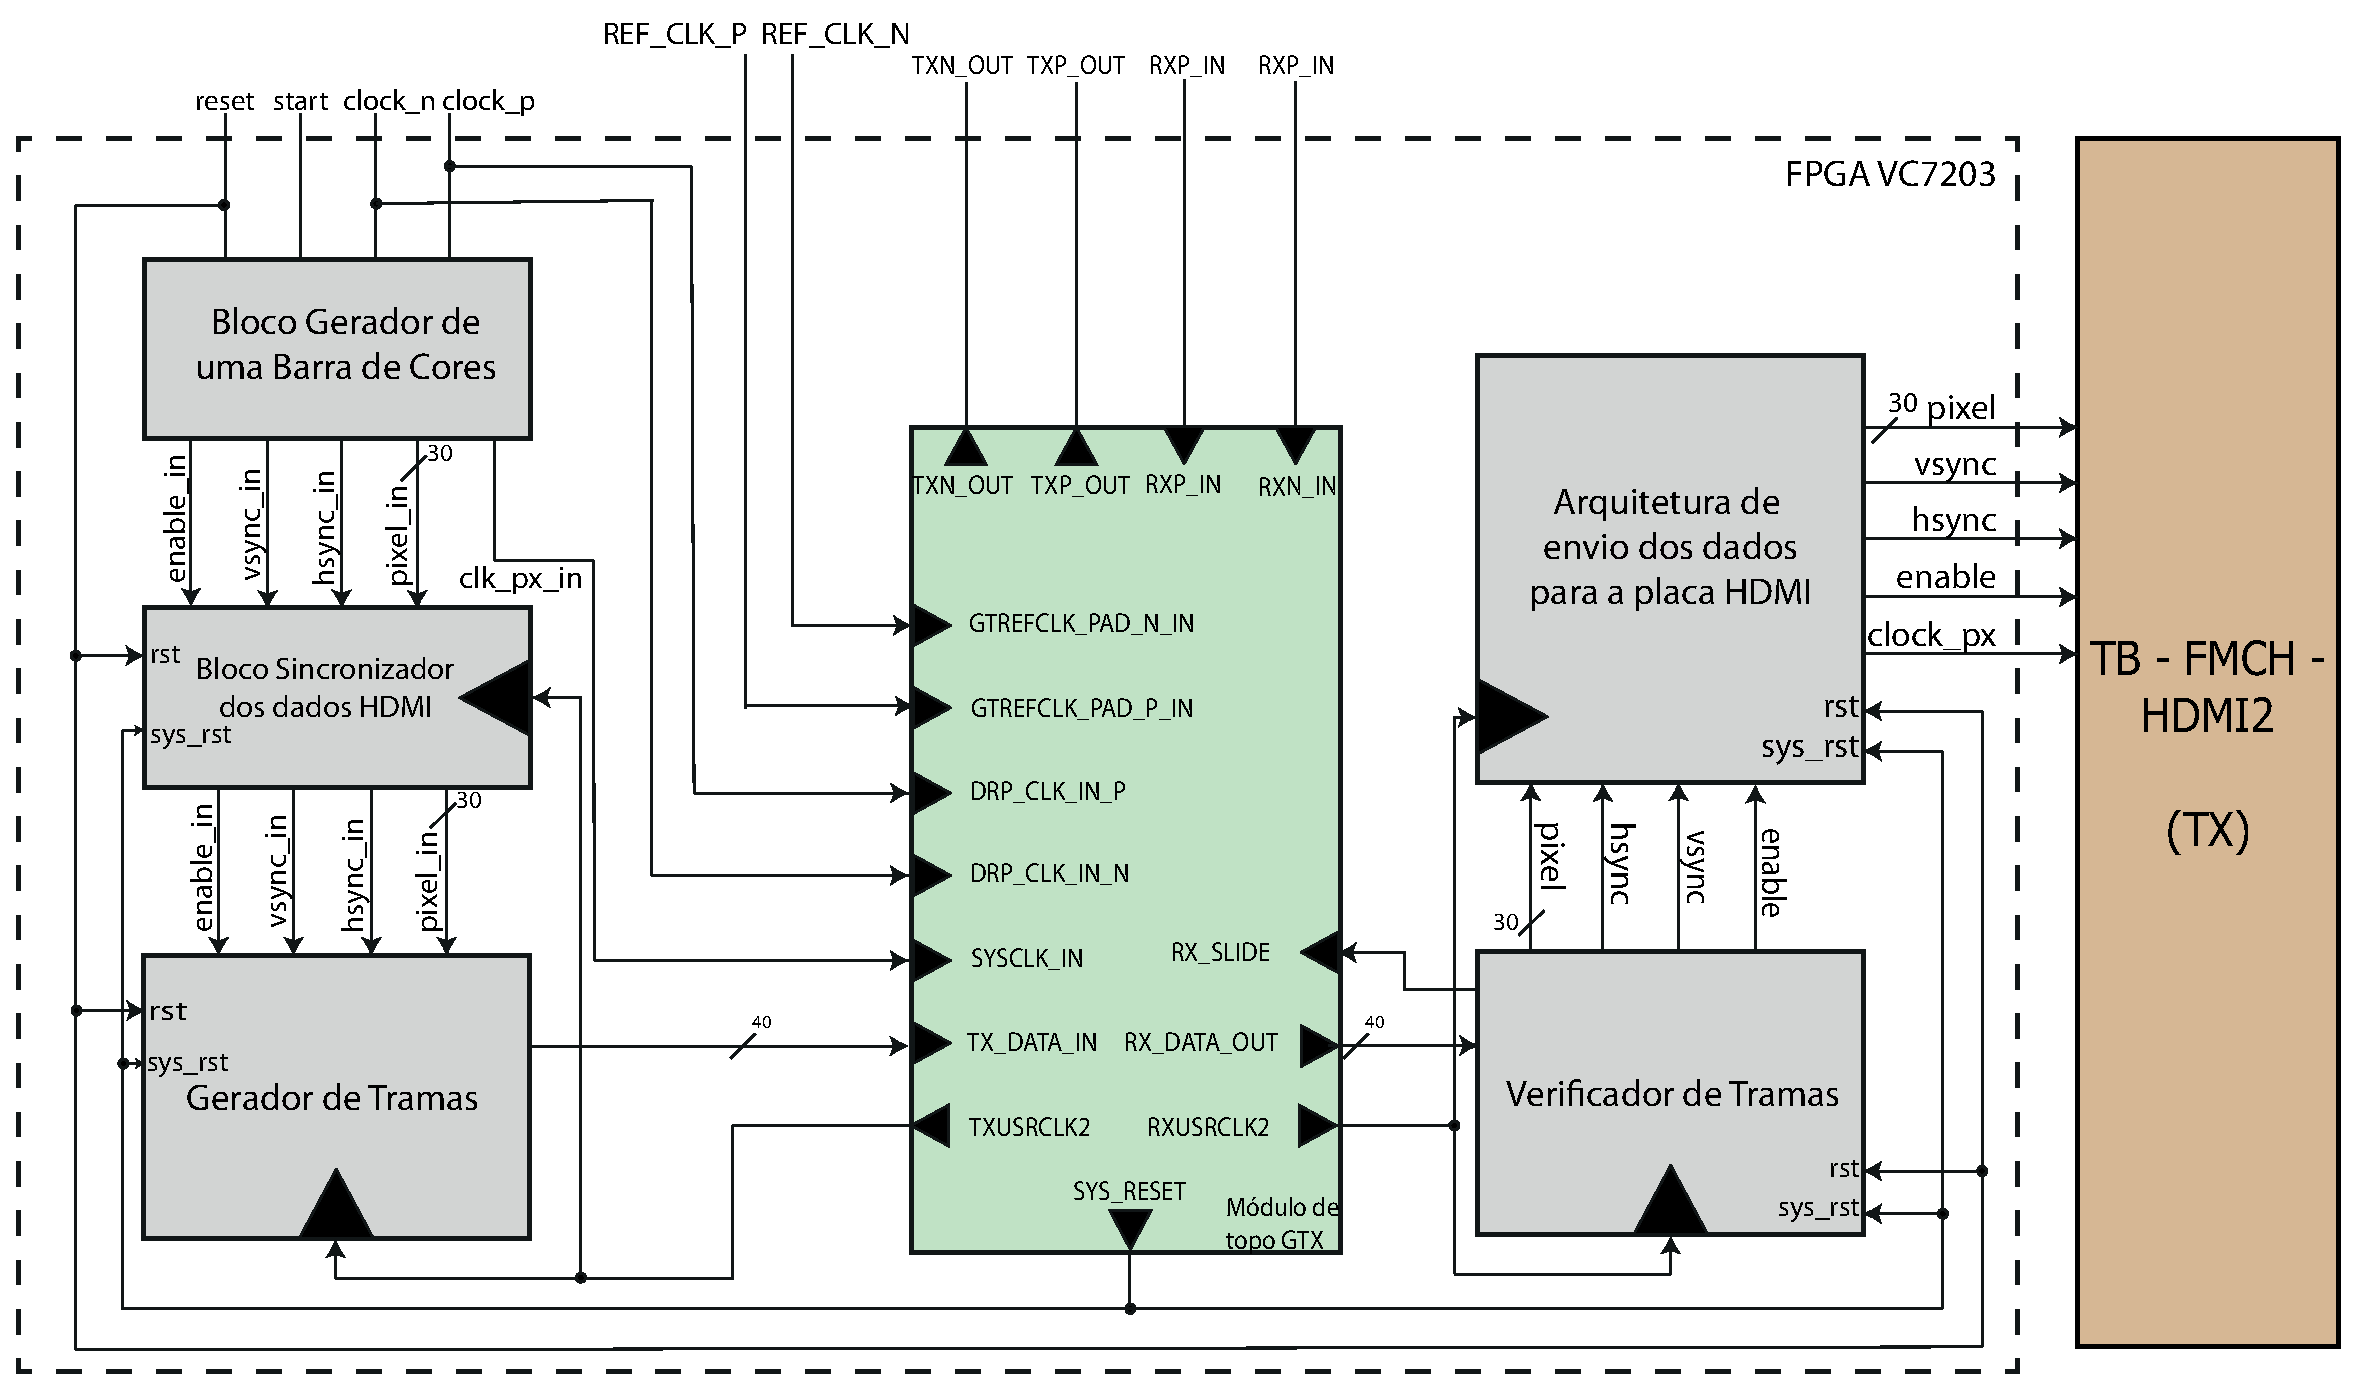
\includegraphics[width=1.0\textwidth]{planod}
		\captionsetup{width=1.0\linewidth}
		\caption[Diagrama de blocos da arquitetura de transmissão em série de uma barra de cores gerada na FPGA]{Diagrama de blocos da arquitetura de transmissão em série de uma barra de cores gerada na FPGA}
		\label{fig:planD}
	\end{center}
\end{figure}

Verifica-se que este bloco tem diversas entradas e saídas, e por isso para além de todo o código desenvolvido em Verilog para estes sub-módulo é necessário definir as localizações físicas da FPGA para cada porta de entrada e saída, estando as mesmas detalhadas na  tabela \ref{table:loc_planD_simples}. Para mais especificações sobre as portas de saída que se conectam à placa HDMI transmissora, remete-se para a secção \ref{ap3:imagemFPGA_TX} do anexo \ref{ap3:LOCs}.

%%%falar das portas todas
\begin{table}[h!]
	\centering
		\caption[Localizações físicas das portas de entrada e saída da arquitetura desenvolvida]{Localizações físicas das portas de entrada e saída da arquitetura desenvolvida}
	\label{table:loc_planD_simples}
	%\resizebox{\textwidth}{!}{%
		\begin{tabular}{rlll}
			\hline
			\multicolumn{1}{l}{}                  & \multicolumn{1}{c}{\textbf{Sinal}} & \multicolumn{1}{c}{\textbf{LOC na FPGA}} & \multicolumn{1}{c}{\textbf{Banco na FPGA}} \\ \hline
			\multicolumn{1}{r|}{\textbf{Entrada}} & clk\_p                             & E19                                      & 38                                         \\
			\multicolumn{1}{r|}{\textbf{Entrada}} & clk\_n                             & E18                                      & 38                                         \\
			\multicolumn{1}{r|}{\textbf{Entrada}} & reset                              & N41                                      & 19                                         \\
			\multicolumn{1}{r|}{\textbf{Entrada}} & start                              & E42                                      & 19                                         \\
			\multicolumn{1}{r|}{\textbf{Entrada}} & REF\_CLK\_P                        & AF8                                      & 114                                        \\
			\multicolumn{1}{r|}{\textbf{Entrada}} & REF\_CLK\_N                        & AF7                                      & 114                                        \\
			\multicolumn{1}{r|}{\textbf{Entrada}} & RXP\_IN                            & AG6                                      & 114                                        \\
			\multicolumn{1}{r|}{\textbf{Entrada}} & RXN\_IN                            & AG5                                      & 114                                        \\
			\multicolumn{1}{r|}{\textbf{Saída}}   & TXN\_OUT                           & AK3                                      & 114                                        \\
			\multicolumn{1}{r|}{\textbf{Saída}}   & TXP\_OUT                           & AK4                                      & 114                                        \\
			\multicolumn{1}{r|}{\textbf{Saída}}   & clk\_px                            & E34                                      & 35                                         \\
			\multicolumn{1}{r|}{\textbf{Saída}}   & enable                             & K35                                      & 34                                         \\
			\multicolumn{1}{r|}{\textbf{Saída}}   & hsync                              & M32                                      & 34                                         \\
			\multicolumn{1}{r|}{\textbf{Saída}}   & vsync                              & L31                                      & 34                                         \\
			\multicolumn{1}{r|}{\textbf{Saída}}   & pixel{[}0{]} a pixel {[}29{]}      & Ver Anexo                                & 34 e 35                                    \\ \hline
		\end{tabular}%
%	}
\end{table}


%%%falar das constraints físicas

O conteúdo do ficheiro de restrições físicas pode ser encontrado nas secções \ref{ap:fisicas_paraHDMI} e \ref{ap:fisicas_planD} do anexo \ref{ap2:codigo}. Na secção \ref{ap:fisicas_paraHDMI}  encontram-se as retrições relativas às portas de saída que se conectam à placa HDMI transmissora e a secção \ref{ap:fisicas_planD} corresponde às restrições físicas das restantes portas desta arquitetura. O conteúdo das restrições temporais desta mesma arquitetura encontra-se na secção \ref{ap:temporais_planD} do anexo \ref{ap2:codigo}.
%
%%%falar das constrainsts temporais
%
\subsubsection{Resultados} \label{subsub:serial_planDresults}

%A arquitetura foi devidamente sintetizada e implementada na FPGA, obtendo-se os resultados dos recursos utilizados para a mesma na tabela \ref{table:recursos_planoD}.
%
%\begin{table}[h!]
%	\centering
%	\caption{Recursos utilizados na FPGA para esta implementação}
%	\label{table:recursos_planoD}
%	\begin{tabular}{llll}
%		\hline
%		\multicolumn{1}{c}{\textbf{Recurso}} & \multicolumn{1}{c}{\textbf{Utilização}} & \multicolumn{1}{c}{\textbf{Disponível}} & \multicolumn{1}{c}{\textbf{Utilização (\%)}} \\ \hline
%		FF                                   & 566                                     & 607200                                  & 0,09                                         \\
%		LUT                                  & 486                                     & 303600                                  & 0,16                                         \\
%		I/O                                  & 44                                      & 700                                     & 6,29                                         \\
%		BUFG                                 & 5                                       & 32                                      & 15,63                                        \\
%	%MMCM                                 & 2                                       & 14                                      & 14,29                                        \\
%		GT                                   & 1                                       & 35                                      & 2,86                                         \\ \hline
%	\end{tabular}
%\end{table}



Após a síntese e implementação da arquitetura desenvolvida a FPGA foi devidamente programada com o \textit{bitstream} gerado. Porém, nesta arquitetura é necessário ter em consideração que o sinal de relógio de referência que se conecta ao GTX é proveniente de um módulo disponível nesta FPGA Virtex-7 com o nome de "\textit{SuperClock2-Module}". Consequentemente, antes da FPGA ser programada com a arquitetura desenvolvida, este módulo deve ser re-programado para a frequência desejada de \SI{148.5}{\mega\hertz}. Para testar a arquitetura utilizou-se o \textit{setup} que se pode visualizar na figura \ref{fig:planD_setup}.
\begin{figure}[h!]
	\begin{center}
		\leavevmode
		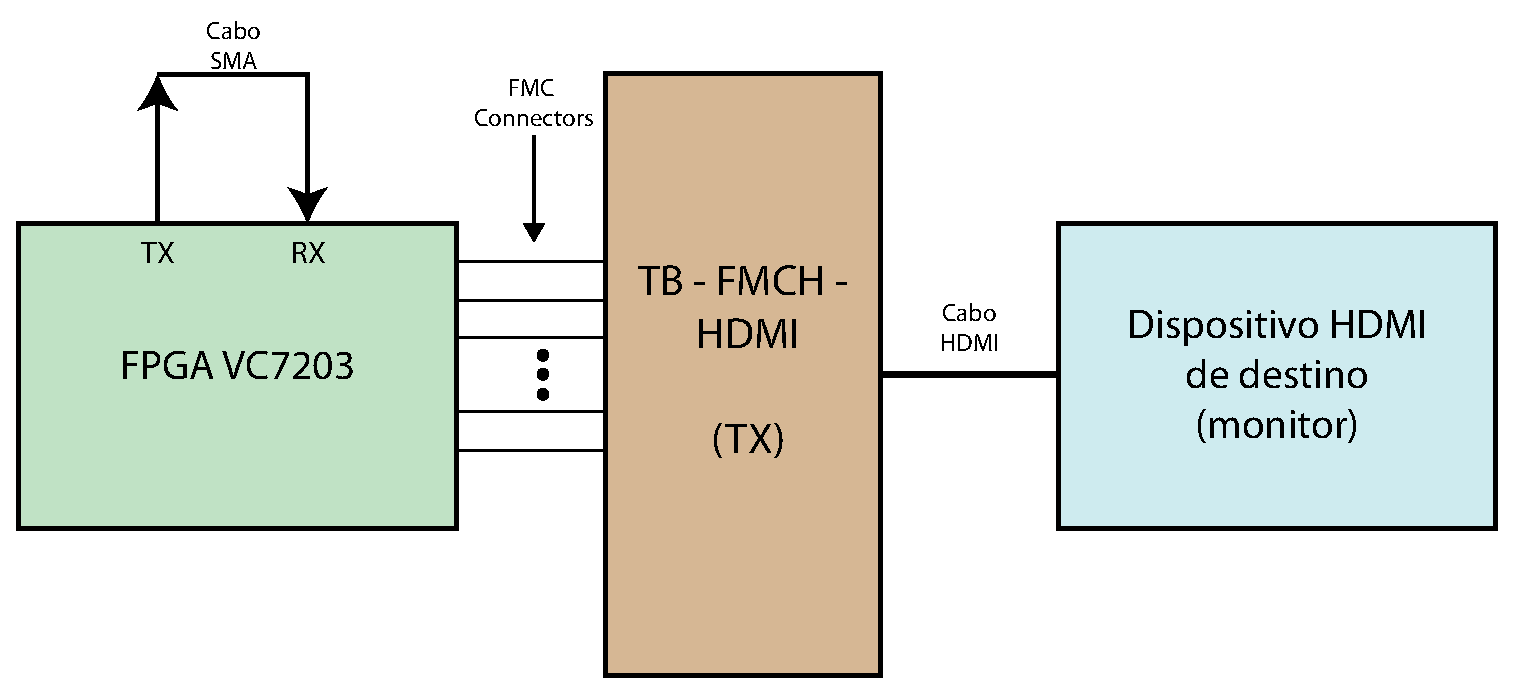
\includegraphics[width=0.8\textwidth]{planDsch}
		\captionsetup{width=1.0\linewidth}
		\caption[\textit{Setup} de teste da arquitetura]{\textit{Setup} de teste da arquitetura de transmissão de dados em série da barra de cores gerada na FPGA}
		\label{fig:planD_setup}
	\end{center}
\end{figure}

\begin{center}
	\lrboxbrace[\Vert][\Vert] {}
	{\textbf{Os resultados obtidos foram os esperados: a transmissão em série foi bem sucedida e visualizou-se uma barra de cores no monitor. Para além disto, quando se desconectam os cabos SMA, a ligação perde-se e quando se voltam a conectar, a mesma é recuperada, o que vem validar a máquina de estados desenvolvida.}}
\end{center}

\begin{figure}[h!]
	\begin{center}
		\leavevmode
		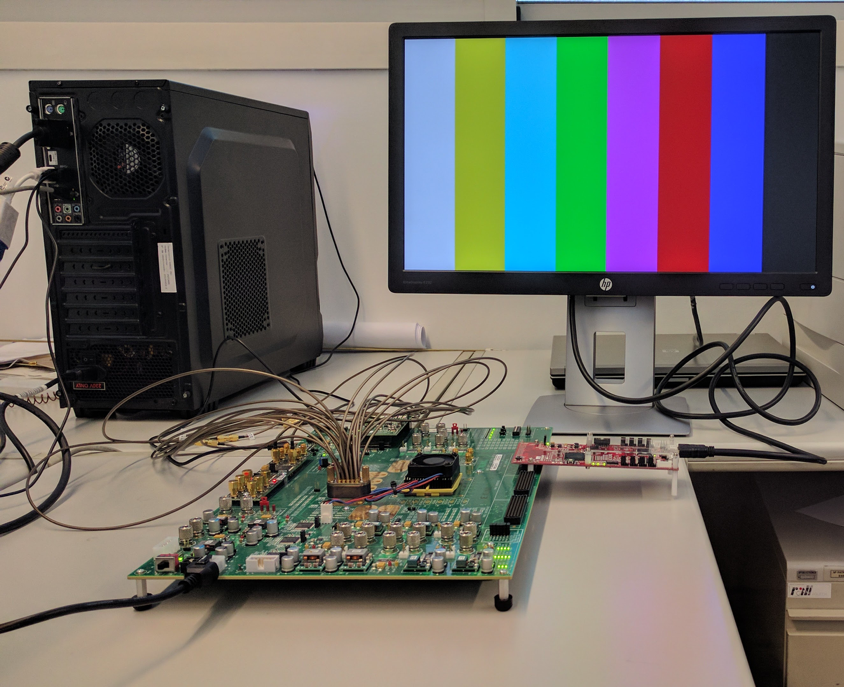
\includegraphics[width=0.7\textwidth]{resultados_planoD}
		\captionsetup{width=1.0\linewidth}
		\caption[Resultados obtidos da transmissão em série de uma barra de cores gerada na FPGA]{Resultados obtidos da transmissão em série de uma barra de cores gerada na FPGA}
		\label{fig:planD_resultados}
	\end{center}
\end{figure}
% \marginpar{ 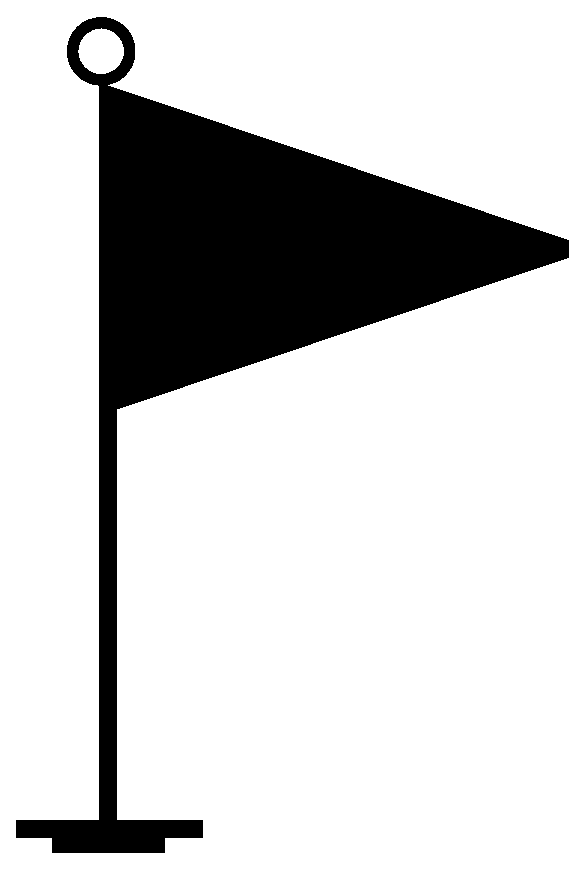
\includegraphics[width=0.5\marginparwidth]{objetivo_cumprido}}



\subsection{Transmissão de imagem em série entre dispositivos HDMI} \label{sub:planE}

Nesta subsecção é apresentada uma arquitetura de transmissão de imagem em série entre dispositivos HDMI. São detalhadas todas as fases de desenvolvimento da arquitetura, todas as decisões tomadas e ainda os resultados obtidos. Esta arquitetura é semelhante à apresentada na subsecção \ref{sub:planD} e por isso muitos dos blocos usados são idênticos aos anteriormente apresentados.

\subsubsection{Considerações sobre a arquitetura} \label{subsub:planE_considerações}

A arquitetura desenvolvida gera uma barra de cores em \textit{FULL HD} na FPGA, tal como anteriormente, e ao mesmo tempo recebe os dados provenientes da placa HDMI recetora. Tal como se visualiza na figura \ref{fig:planE_simples}, os dados a ser transmitidos vão depender do valor de "\textit{start}". Este sinal define a seleção do multiplexador que se visualiza na figura: se estiver ativo seleciona os dados provenientes do módulo gerador da barra de cores, se estiver inativo os dados selecionados pelo multiplexador são os dados provenientes da placa HDMI recetora.

\begin{figure}[h!]
	\begin{center}
		\leavevmode
		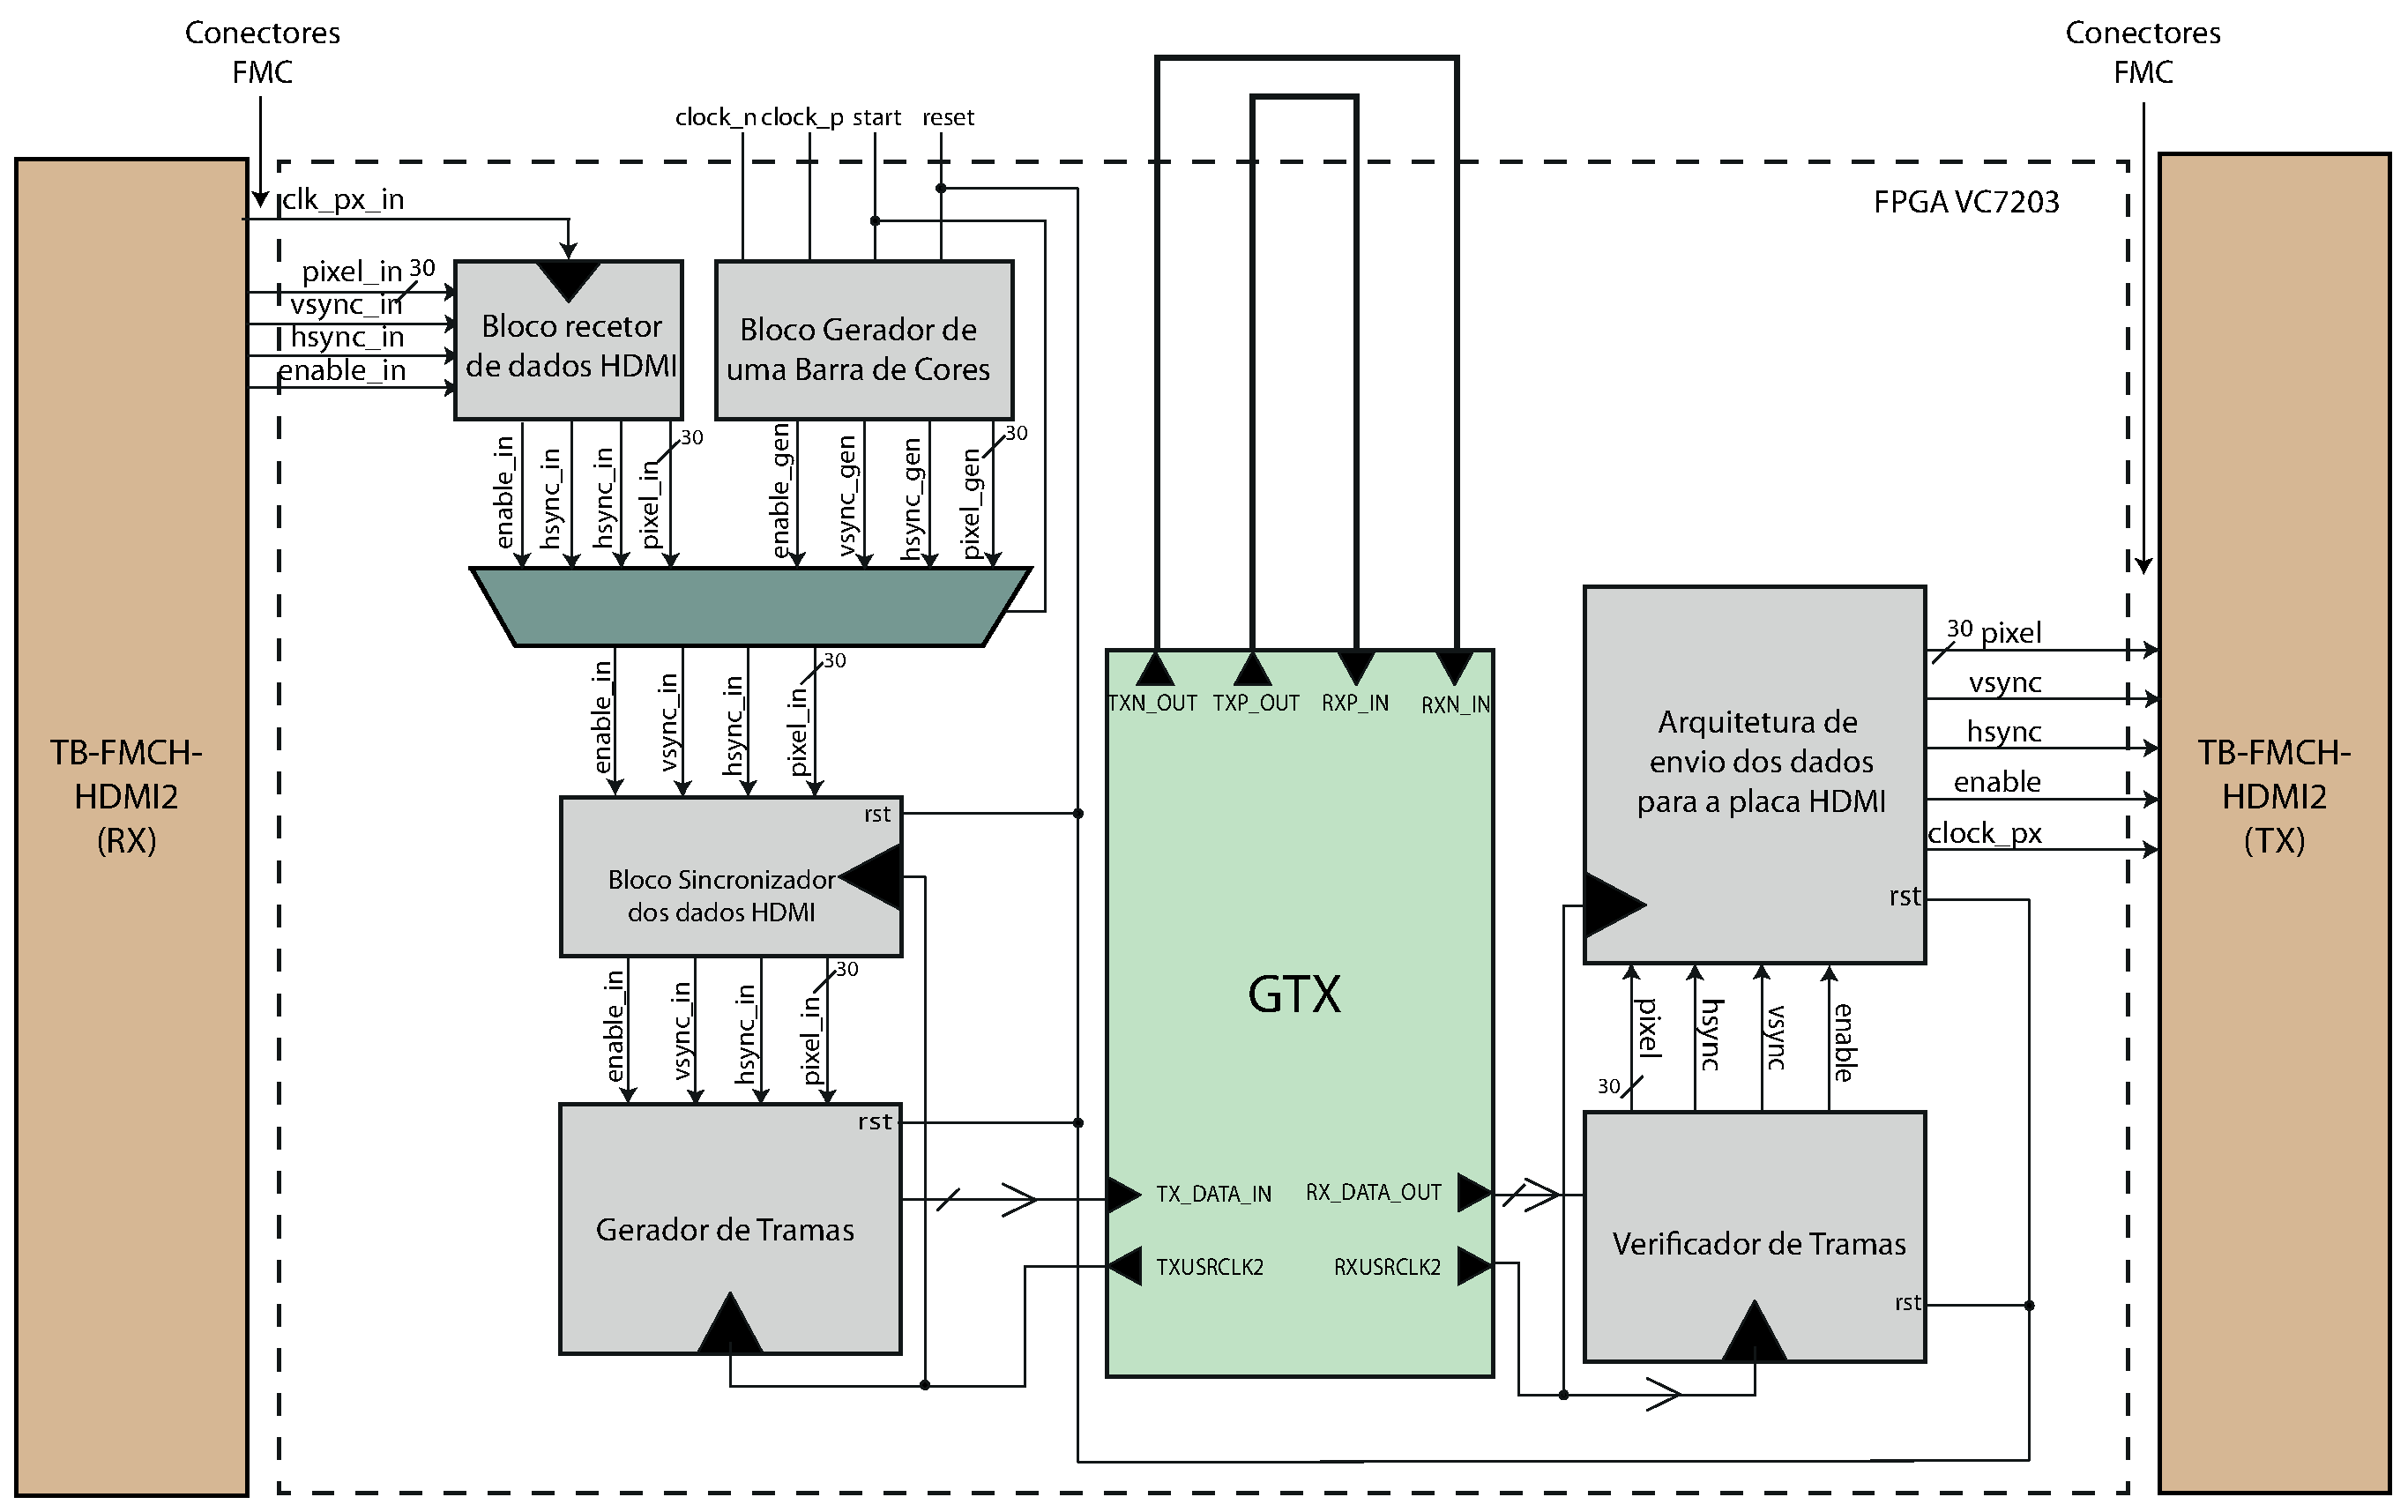
\includegraphics[width=1.0\textwidth]{planoE_simples_pt}
		\captionsetup{width=1.0\linewidth}
		\caption[Diagrama geral da arquitetura de transmissão em série de imagem entre dispositivos HDMI]{Diagrama geral da arquitetura de transmissão em série de imagem entre dispositivos HDMI}
		\label{fig:planE_simples}
	\end{center}
\end{figure}


\subsubsection{Conceção e Desenvolvimento}

Através da visualização do diagrama blocos simplificado apresentado na figura \ref{fig:planE_simples} é possivel concluir que o único sub-módulo adicionado é o bloco recetor de dados HDMI. Todos os outros sub-módulos são exatamente iguais ao da arquitetura anterior, estando detalhados na subsecção \ref{sub:planD}. Assim sendo, apenas será apresentado nesta subsecção esse mesmo bloco.

\subsubsection*{Bloco Recetor de dados HDMI}
%explicar o que faz
O bloco recetor de dados HDMI recebe os dados provenientes da placa recetora e guarda-os em registos síncronos com o flanco positivo do sinal de relógio proveniente da mesma. O diagrama de blocos deste módulo visualiza-se na figura \ref{fig:recetorHDMI}.
%explicar o porque de ser necessário
\begin{figure}[h!]
	\begin{center}
		\leavevmode
		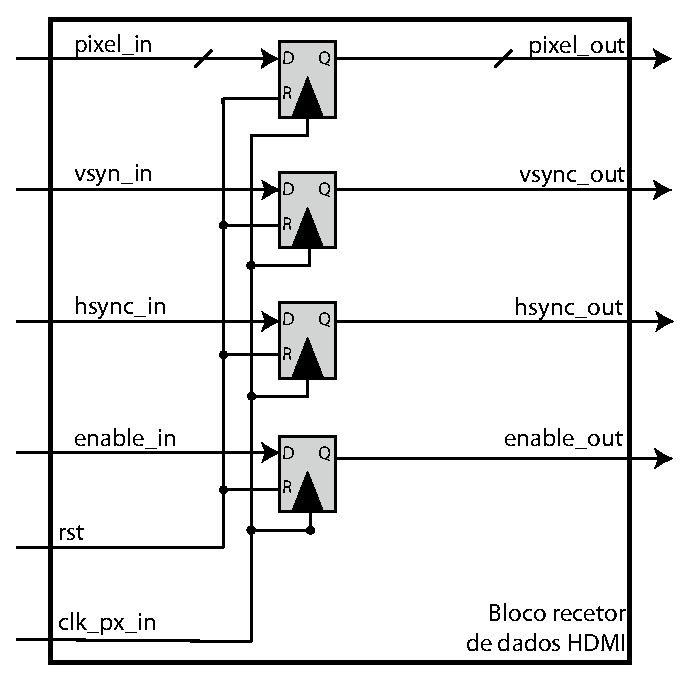
\includegraphics[width=0.4\textwidth]{recetorHDMI}
		\captionsetup{width=1.0\linewidth}
		\caption[Bloco recetor de dados HDMI]{Bloco Recetor de dados HDMI}
		\label{fig:recetorHDMI}
	\end{center}
\end{figure}

É de relembrar que existem dois domínios de relógio principais quando se faz a transmissão de dados entre a placa HDMI recetora para o transcetor GTX: o sinal de relógio proveniente da placa HDMI e o sinal de relógio proveniente do transcetor. Apesar de já existir um bloco responsável pela sincronização de dados do domínio do sinal de relógio TXUSRCLK2, o autor de \cite{R024} recomenda que também haja sincronização do lado do domínio que envia os dados. Apesar de as saídas da placa HDMI serem amostradas a uma determinada cadência, segundo os manuais das mesmas (\cite{R009}, \cite{R014} e \cite{R013}), pode existir algum desfasamento de dados que possa vir a provocar meta-estabilidade. Assim sendo, optou-se por criar este bloco.

\subsubsection*{Localizações das portas de saída do módulo de topo} \label{subsub:serial_locs_planE}

Na figura \ref{fig:planoE} encontra-se o diagrama de blocos da arquitetura desenvolvida para a transmissão de imagem em série entre dispositivos HDMI. A mesma ilustra os blocos desenvolvidos para a sua conceção referindo as principais portas de entrada e saída.

\begin{figure}[h!]
	\begin{center}
		\leavevmode
		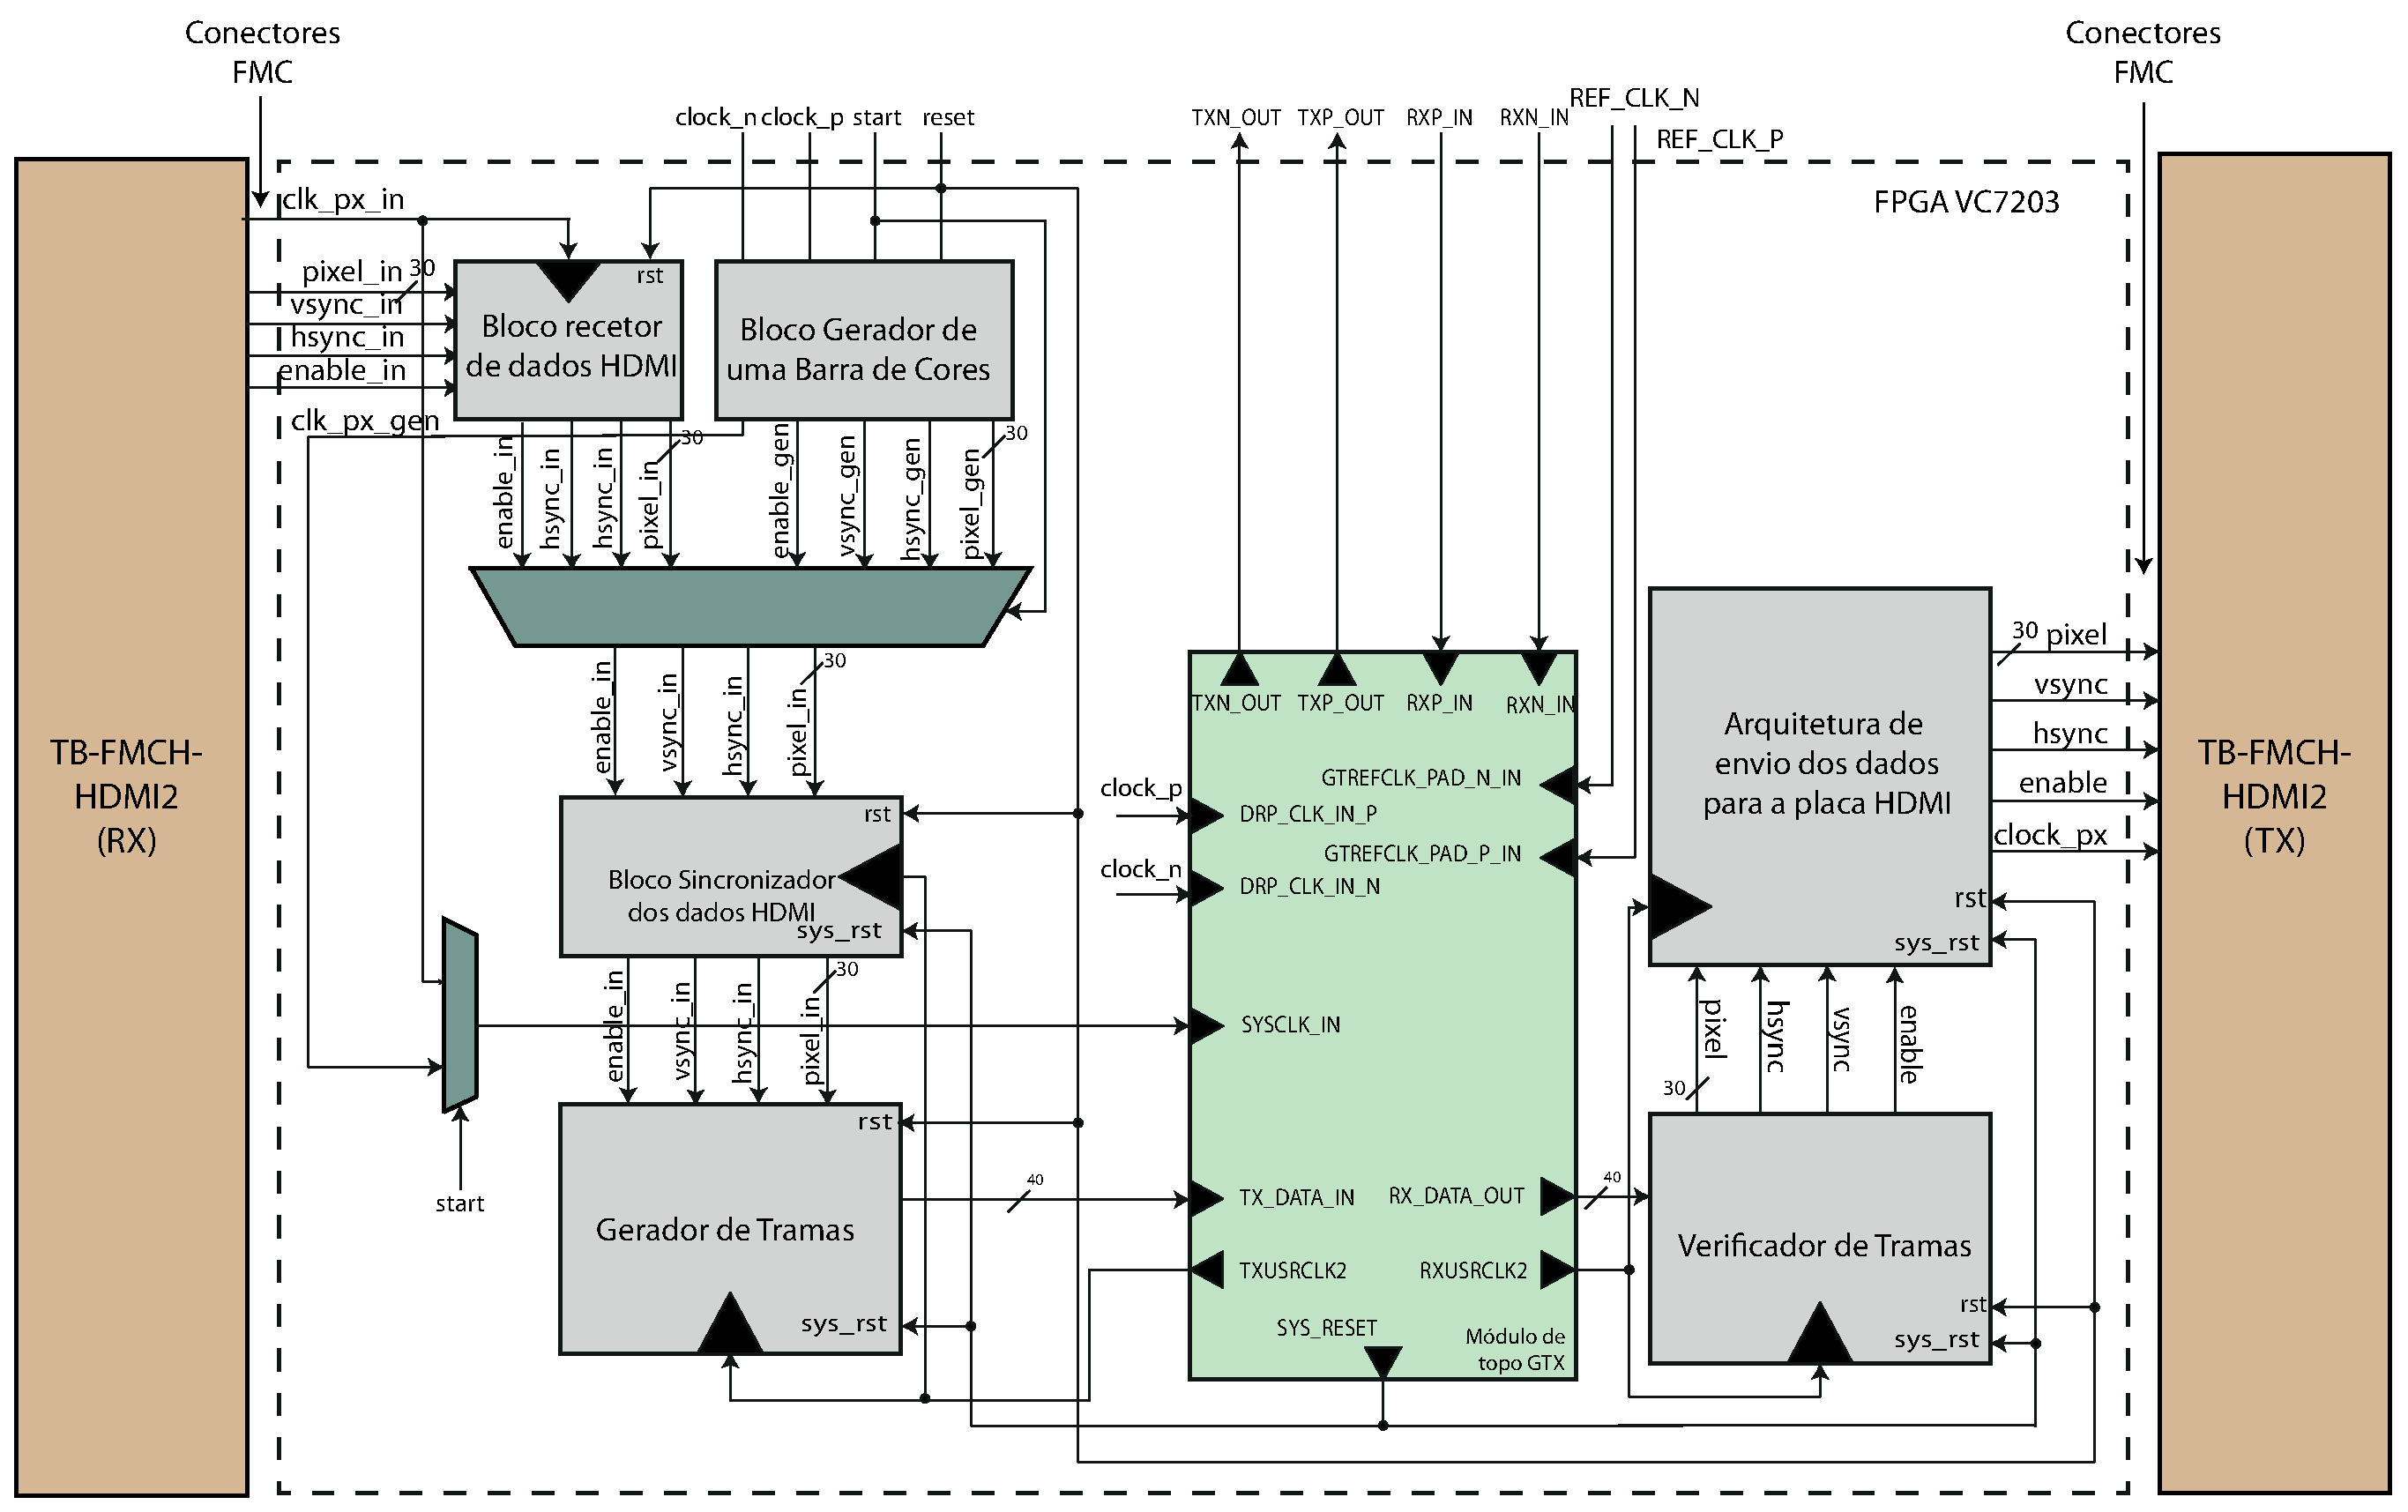
\includegraphics[width=1.0\textwidth]{planoE}
		\captionsetup{width=1.0\linewidth}
		\caption[Diagrama de blocos da arquitetura de transmissão de imagem em série]{Diagrama de blocos da arquitetura de transmissão de imagem em série}
		\label{fig:planoE}
	\end{center}
\end{figure}

As localizações físicas das portas de entrada e saída do bloco encontram-se detalhadas na tabela \ref{table:LOC_simples_planE}. Como se pode observar, existem algumas portas que não estão representadas na figura \label{fig:planE} para simplificá-la. Essas portas são provenientes do módulo verificador de tramas e a sua principal função é manter o utilizador a par dos estados da transmissão do lado do recetor.  As mesmas são referidas na tabela com os nomes de "\textit{begin\_state}", "\textit{SOP\_detected}", "\textit{track\_data}", "\textit{data\_error\_detected }", "\textit{idle\_slip }", "\textit{wait\_state}" e "\textit{align}" e correspondem aos diferentes estados da máquina apresentada na secção \ref{subsub:serial_frameChecker} na página \pageref{subsub:serial_frameChecker}.

\begin{table}[h!]
	\centering
	\caption{Localizações físicas das portas de entrada e saída da arquitetura}
	\label{table:LOC_simples_planE}
	\begin{tabular}{rlll}
		\hline
		\multicolumn{1}{l}{}                  & \multicolumn{1}{c}{\textbf{Sinal}}     & \multicolumn{1}{c}{\textbf{LOC na FPGA}} & \multicolumn{1}{c}{\textbf{Banco na FPGA}} \\ \hline
		\multicolumn{1}{r|}{\textbf{Entrada}} & clk\_p                                 & E19                                      & 38                                         \\
		\multicolumn{1}{r|}{\textbf{Entrada}} & clk\_n                                 & E18                                      & 38                                         \\
		\multicolumn{1}{r|}{\textbf{Entrada}} & reset                                  & N41                                      & 19                                         \\
		\multicolumn{1}{r|}{\textbf{Entrada}} & start                                  & E42                                      & 19                                         \\
		\multicolumn{1}{r|}{\textbf{Entrada}} & REF\_CLK\_P                            & AF8                                      & 114                                        \\
		\multicolumn{1}{r|}{\textbf{Entrada}} & REF\_CLK\_N                            & AF7                                      & 114                                        \\
		\multicolumn{1}{r|}{\textbf{Entrada}} & RXP\_IN                                & AG6                                      & 114                                        \\
		\multicolumn{1}{r|}{\textbf{Entrada}} & RXN\_IN                                & AG5                                      & 114                                        \\
		\multicolumn{1}{r|}{\textbf{Entrada}} & clk\_px\_in                            & AJ32                                     & 14                                         \\
		\multicolumn{1}{r|}{\textbf{Entrada}} & enable\_in                             & AN38                                     & 15                                         \\
		\multicolumn{1}{r|}{\textbf{Entrada}} & hsync\_in                              & AU39                                     & 15                                         \\
		\multicolumn{1}{r|}{\textbf{Entrada}} & vsync\_in                              & AU38                                     & 15                                         \\
		\multicolumn{1}{r|}{\textbf{Entrada}} & pixel\_in {[}0{]} a pixel\_in {[}29{]} & Ver Anexo                                & 14 e 15                                    \\
		\multicolumn{1}{r|}{\textbf{Saída}}   & TXN\_OUT                               & AK3                                      & 114                                        \\
		\multicolumn{1}{r|}{\textbf{Saída}}   & TXP\_OUT                               & AK4                                      & 114                                        \\
		\multicolumn{1}{r|}{\textbf{Saída}}   & begin\_state                           & M38                                      & 19                                         \\
		\multicolumn{1}{r|}{\textbf{Saída}}   & SOP\_detected                          & R42                                      & 19                                         \\
		\multicolumn{1}{r|}{\textbf{Saída}}   & track\_data                            & P42                                      & 19                                         \\
		\multicolumn{1}{r|}{\textbf{Saída}}   & data\_error\_detected                  & N38                                      & 19                                         \\
		\multicolumn{1}{r|}{\textbf{Saída}}   & idle\_slip                             & M39                                      & 19                                         \\
		\multicolumn{1}{r|}{\textbf{Saída}}   & wait\_state                            & R40                                      & 19                                         \\
		\multicolumn{1}{r|}{\textbf{Saída}}   & align                                  & P40                                      & 19                                         \\
		\multicolumn{1}{r|}{\textbf{Saída}}   & clk\_px                                & E34                                      & 35                                         \\
		\multicolumn{1}{r|}{\textbf{Saída}}   & enable                                 & K35                                      & 34                                         \\
		\multicolumn{1}{r|}{\textbf{Saída}}   & hsync                                  & M32                                      & 34                                         \\
		\multicolumn{1}{r|}{\textbf{Saída}}   & vsync                                  & L31                                      & 34                                         \\
		\multicolumn{1}{r|}{\textbf{Saída}}   & pixel{[}0{]} a pixel {[}29{]}          & Ver Anexo                                & 34 e 35                                    \\ \hline
	\end{tabular}
\end{table}

As portas que estão diretamente ligadas às placas HDMI (tanto à de transmissão como à de receção) encontram-se pouco detalhadas nesta tabela. No entanto, na secção \ref{ap3:imagem_RX_TX} do anexo \ref{ap3:LOCs} é possível encontrar as mesmas com mais detalhe, tanto do lado da FPGA como do lado das placas HDMI.

%constraints fisicas
O conteúdo do ficheiro de restrições físicas encontra-se nas secções \ref{ap:fisicas_deHDMI}, \ref{ap:fisicas_paraHDMI} e \ref{ap:fisicas_planE} do anexo \ref{ap2:codigo}. Na secção \ref{ap:fisicas_deHDMI} encontram-se as restrições físicas referentes às portas de entrada que se conectam à placa HDMI recetora. Na secção \ref{ap:fisicas_paraHDMI} referentes às portas de saída da arquitetura que se conectam à placa HDMI transmissora. Por fim, na secção \ref{ap:fisicas_planE} encontram-se as restrições físicas das restantes portas desta arquitetura. O conteúdo referente às restrições temporais da mesma encontram-se na secção \ref{ap:temporais_planE} do anexo \ref{ap2:codigo}.
%constraints temporais

\subsubsection{Resultados} \label{subsub:serial_planEresults}

%A arquitetura foi devidamente sintetizada e implementada na FPGA, obtendo-se os seguintes resultados resumidos apresentados na tabela \ref{table:recursos_planoE} relativamente aos recursos utilizados na mesma. 

%\begin{table}[h!]
%	\centering
%	\caption{Recursos utilizados na implementação da arquitetura}
%	\label{table:recursos_planoE}
%
%		\begin{tabular}{llll}
%			\hline
%			\multicolumn{1}{c}{\textbf{Recurso}} & \multicolumn{1}{c}{\textbf{Utilização}} & \multicolumn{1}{c}{\textbf{Disponível}} & \multicolumn{1}{c}{\textbf{Utilização (\%)}} \\ \hline
%			FF                                   	& 710                                     & 607200                                  & 0,12                                         \\
%			LUT                                  & 590                                     & 303600                                  & 0,19                                         \\
%			Memory LUT                           & 6                                       & 130800                                  & 0,01                                         \\
%			I/O                                  & 78                                      & 700                                     & 11,14                                        \\
%			BUFG                                 & 2                                       & 32                                      & 6,25                                         \\
%			GT                                   & 1                                       & 35                                      & 2,86                                         \\ \hline
%		\end{tabular}%
%
%\end{table}

	
%Tal como é de esperar, esta é a arquitetura que utiliza mais recursos comparativamente às outras todas desenvolvidas, no entanto ainda existem muitos disponíveis.	
%setup da cena


A arquitetura desenvolvida foi devidamente sintetizada e implementada na FPGA, e para se proceder ao teste da mesma utilizou-se o \textit{setup} que se visualiza na figura \ref{fig:planoE_setup}. Conectam-se os dispositivo HDMI de fonte e de destino às placas HDMI, que por sua vez estão conectados à FPGA que permite fazer a transmissão em série de imagem entre ambos.

\begin{figure}[h!]
	\begin{center}
		\leavevmode
		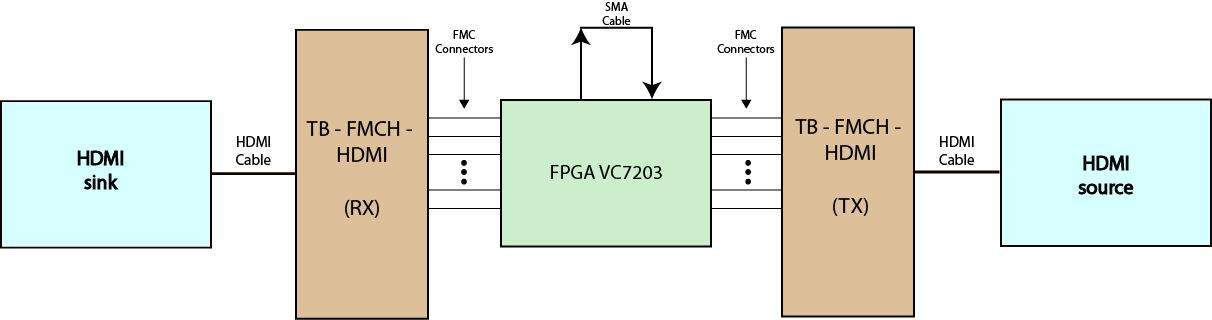
\includegraphics[width=0.9\textwidth]{planEsch_en}
		\captionsetup{width=1.0\linewidth}
		\caption[\textit{Setup} de teste para a arquitetura de transmissão em série entre dispositivos HDMI]{\textit{Setup} de teste para a arquitetura de transmissão em série entre dispositivos HDMI}
		\label{fig:planoE_setup}
	\end{center}
\end{figure}

%explicar resultados

Obteve-se uma transmissão em série como pretendido entre ambos os dispositivos, mas surgiu um problema. Apesar de nas diversas simulações realizadas (funcional, pós-síntese e pós-implementação) a arquitetura ter sido validada, quando se implementa a mesma na FPGA ocorre um problema de visualização da imagem no dispositivo de destino: são apresentadas umas ligeiras riscas pretas horizontais. O resultado está apresentado na figura \ref{fig:planoE_results}.


\begin{figure}
	\begin{center}
	\leavevmode
	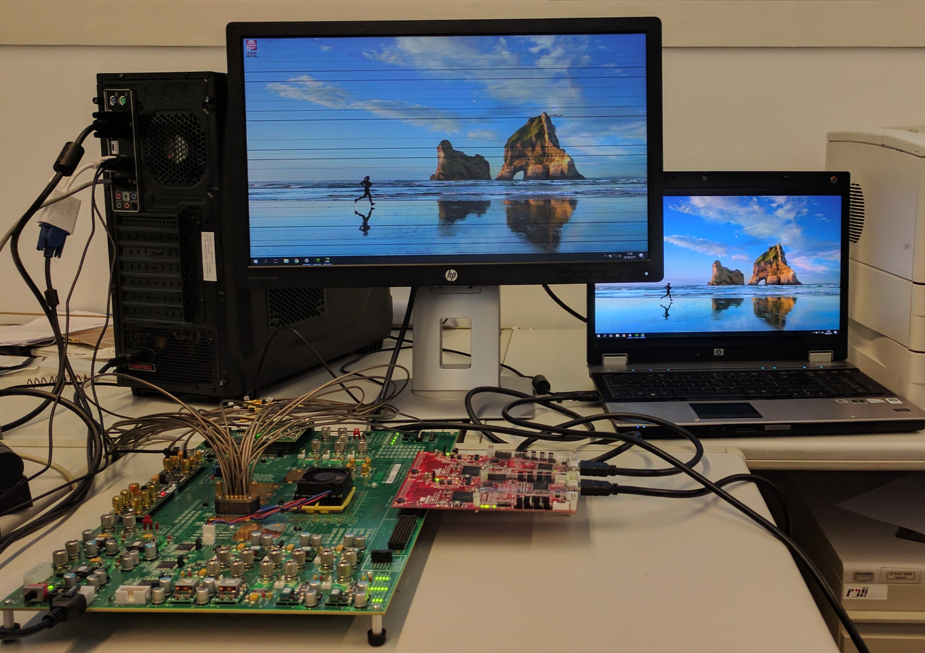
\includegraphics[width=0.7\textwidth]{resultados_planoE}
	\captionsetup{width=1.0\linewidth}
	\caption[Resultado obtido da arquitetura de transmissão em série entre dispositivos HDMI]{Resultado obtido da arquitetura de transmissão em série entre dispositivos HDMI}
	\label{fig:planoE_results}
\end{center}
\end{figure}

%explicar problema
O problema foi diagnosticado recorrendo-se à utilização de um \textit{IP} da Xilinx, designado por ILA (\textit{Integrated Logic Analyzer}), que permite monitorizar os sinais internos da FPGA através das suas diversas características tendo como base de tempo o sinal de relógio de referência do mesmo. O problema não se deve à transmissão em série, mas sim a uma falha sincronização entre registos antes de se realizar a mesma.

\begin{figure}
	\begin{center}
		\leavevmode
		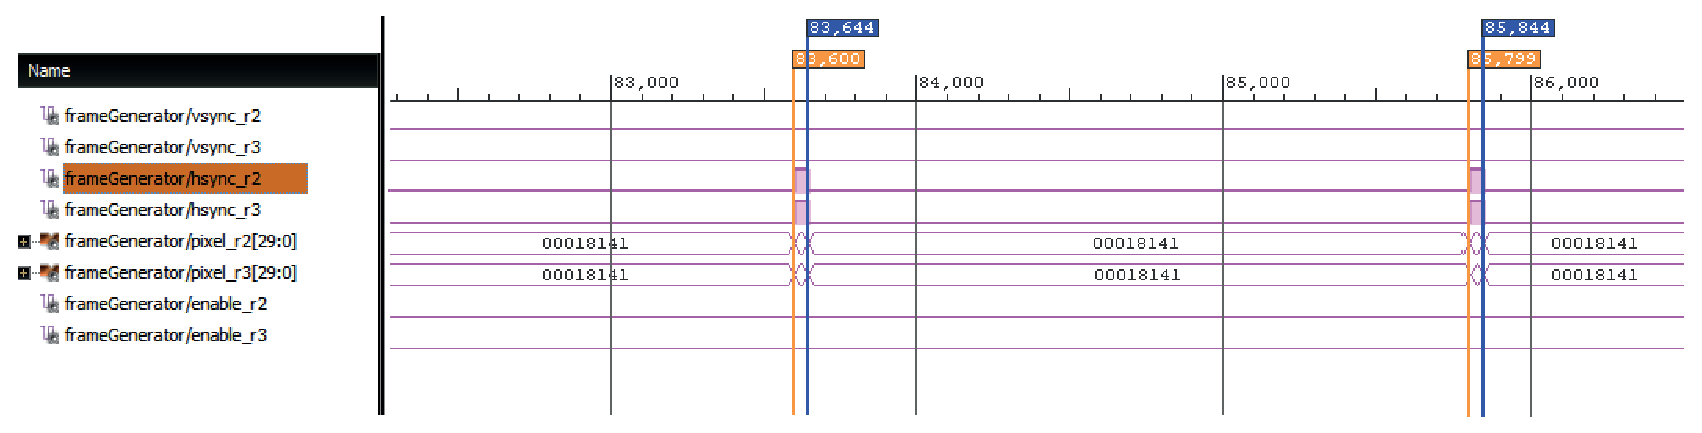
\includegraphics[width=1.0\textwidth]{erro_planoE}
		\captionsetup{width=1.0\linewidth}
		\caption[Gráfico da análise do comportamento dos sinais internos da FPGA]{Gráfico da análise do comportamento dos sinais internos da FPGA}
		\label{fig:planoE_rerro}
	\end{center}
\end{figure}

Na figura \ref{fig:planoE_rerro} é possível visualizar um gráfico retirado da análise dos sinais internos da FPGA. De notar que a base de tempo é o sinal de relógio de referência, que para este caso foi TXUSRCLK2 (proveniente do GTX), e por isso uma unidade na figura representa um ciclo de relógio do mesmo.  Neste gráfico estão a ser analisadas as transições dos dados do sub-módulo do sistema "Bloco Recetor de dados HDMI" para o "Bloco Sincronizador dos dados HDMI". Os sinais "\textit{hsync\_r2}" e "\textit{hsync\_r3}" no gráfico correspondem aos dois registos de sincronização do bloco "Sincronizador dos dados HDMI" ilustrado na figura \ref{fig:sync_block}.

O que está a causar o problema, através da análise feita, é a falha num ciclo de relógio de uma linha inteira. Ou seja, na primeira transição que se vê no sinal \textit{hsync\_r2} o seu comportamento é como esperado: tem um tempo de duração de 44 ciclos de relógio e encontra-se no início da transmissão de uma linha completa. No entanto, na segunda transição do mesmo o seu comportamento não é o esperado: tem um tempo de duração de 45 ciclos de relógio e fica ativo um ciclo de relógio antes do início da linha. Relembrando que uma linha completa tem 2200 ciclos de relógio, a diferença entre a primeira transição de 0 para 1 do sinal em questão para a segunda é de 2199 ciclos de relógio. 

Este problema acaba por acontecer em várias linhas causando uma falha na sincronização horizontal da imagem, o que provoca as ligeiras riscas pretas que se visualizam na imagem recebida.

%explicar como soluccionar o problema

Assim, conclui-se que apesar da transmissão em série estar a operar como esperado, o processo de transmissão de dados não é robusto. Os sinais são transmitidos diretamente e apesar de ter havido precauções quanto ao sincronismo entre os domínios de relógio, existiu uma falha de sincronismo.

\begin{center}
	\lrboxbrace[\Vert][\Vert] {} {
\textbf{Em suma, o trabalho desenvolvido até agora relativamente à transmissão de dados em série está validado. Contudo esta arquitetura apresenta um ligeiro problema, cuja solução passa por controlar a transmissão dos dados de sincronismo da imagem de uma maneira diferente. \\ A criação de pacotes com tramas definidas para todos os momentos da transmissão é uma das soluções para o problema.}
}
\end{center}


\subsection{Análise dos recursos utilizados por cada uma das arquiteturas}

Nesta subsecção são apresentadas comparações relativamente aos recursos utilizados na FPGA por cada uma das arquiteturas. Por questões de simplificação definiu-se:
\begin{itemize}
	\item \textbf{Arquitetura D:} Arquitetura transmissora de uma barra de cores em série para o dispositivo final HDMI;
	\item \textbf{Arquitetura E:} Arquitetura transmissora de imagem em série entre dispositivos HDMI;
\end{itemize}

\begin{table}[h!]
	\centering
	\caption{Recursos utilizados pelas arquiteturas desenvolvidas de transmissão em série}
	\label{table:recursos_planoD_planoE}

		\begin{tabular}{rllll}
			\hline
			\multicolumn{1}{c}{\multirow{2}{*}{\textbf{Recurso}}} & \multicolumn{2}{c}{\textbf{Arquitetura D}}                                 & \multicolumn{2}{c}{\textbf{Arquitetura E}}                               \\ \cline{2-5} 
			\multicolumn{1}{c}{}                                  & \multicolumn{1}{c}{\textbf{Utilização}} & \multicolumn{1}{c|}{\textbf{\%}} & \multicolumn{1}{c}{\textbf{Utilização}} & \multicolumn{1}{c}{\textbf{\%}} \\ \hline
			\multicolumn{1}{r|}{\textbf{FF}}                      & 566                                     & \multicolumn{1}{l|}{0,09}        & 710                                    & 0,12                            \\
			\multicolumn{1}{r|}{\textbf{LUT}}                     & 486                                     & \multicolumn{1}{l|}{0,16}        & 590                                    & 0,19                            \\
			\multicolumn{1}{r|}{\textbf{I/O}}                     & 44                                      & \multicolumn{1}{l|}{6,29}        & 78                                     & 11,14                           \\
			\multicolumn{1}{r|}{\textbf{GT}}                      & 1                                       & \multicolumn{1}{l|}{2,86}        & 1                                      & 2,86                            \\ \hline
		\end{tabular}%
\end{table}

Na tabela \ref{table:recursos_planoD_planoE} são apresentados a utilização de recursos de cada uma das arquiteturas, sendo que estes dados foram retirados do \textit{software} após implementação de ambas as arquiteturas.

Globalmente, a arquitetura E utiliza mais recursos do que a D devido ao facto de suportar a receção de dados provenientes da placa HDMI recetora (aumentando o número de entradas e saída utilizadas), e também de utilizar mais um bloco (o que aumenta o número de utilização de FF e LUT). Ambas utilizam apenas um GT (\textit{Gigabit Transceiver}), tal como esperado, havendo ainda a possibilidade de aumentar essa utilização caso se pretenda.

Num ponto de vista geral, a utilização de recursos não se torna preocupante nesta FPGA, havendo ainda muitos recursos disponíveis caso se pretenda abordar estas arquiteturas de maneira diferente.